% -------------------------------------------------------------------------------------------------
%
%  Skeleton for theses at the Institute of Robotics and Intelligent Systems
%
% -------------------------------------------------------------------------------------------------
%
% FILENAME:   thesis.tex
%
% ABSTRACT:   main file for theses
%
% EXCEPTIONS: -
%
% USAGE:      !!!!!!COMPILE WITH PDFLATEX, *NOT* WITH LATEX OR TEX!!!!!!!
%
% HISTORY:    written by Sascha A. Stoeter <stoeter@iris.ethz.ch>, www.stoeter.com, 02.06.2004
%             modified by Martin Probst, 18.08.2004
%             modified by Chauncey Graetzel, 11.05.2005

% -------------------------------------------------------------------------------------------------

\documentclass[12pt,a4paper,onecolumn]{article}
\usepackage{irisarticle}

% -------------------------------------------------------------------------------------------------
% Add needed packages. Some generally useful packages are listed for
% your convenience.
% -------------------------------------------------------------------------------------------------
\usepackage{subfigure}                          % enable the use of subfigures
%\usepackage[bf]{caption}                       % must go after subfigure
\usepackage[thickspace,thinqspace]{SIunits}     %

\usepackage{hyperref}                           % enable Hyperlinks in pdf/ps Docs
\usepackage{pdfpages}
\usepackage{todonotes}



% -------------------------------------------------------------------------------------------------
% Some handy definition to simplify future markup changes
% -------------------------------------------------------------------------------------------------
\providecommand{\eg}{e.g.}
\providecommand{\etal}{\textit{et al.}}
\providecommand{\ie}{i.e.}

%\setlength{\textwidth}{18cm} \setlength{\oddsidemargin}{-1cm}
%\setlength{\evensidemargin}{-1cm}

% -------------------------------------------------------------------------------------------------
% Select type of thesis
% -------------------------------------------------------------------------------------------------
\renewcommand{\iristhesistype}{Bachelor}

% -------------------------------------------------------------------------------------------------
% Set names
% -------------------------------------------------------------------------------------------------
\renewcommand{\irisauthor}{Berk Nergiz}
%:
\renewcommand{\irisadviser}{}


% -------------------------------------------------------------------------------------------------
% Beginning of the main document body
% -------------------------------------------------------------------------------------------------
\begin{document}

% include all Bib-items even if they're not cited in the text
\nocite{*}

% This is the first part of the front matter. Pages appear unnumbered
% and the pages are not counted.

% Title page: set title and date preferably formatted according to
% ISO 8601
\iristitlepage{1D Computations of Flow and Oxygen Transport in Micro-Vascular Networks}{June 2018}


% This is the second part of the front matter. Pages appear with
% lowercase roman numbering. The first page number is 'i'.
\pagenumbering{roman}

% Table of contents
\newpage
\tableofcontents
\addtocontents{toc}{\vspace{.5\baselineskip}}

% List of tables
%\newpage
%\addcontentsline{toc}{section}{\protect\numberline{}{List of Tables}}
%\listoftables

% List of figures
%\newpage
%\addcontentsline{toc}{section}{\protect\numberline{}{List of Figures}}
%\listoffigures

\clearpage
\pagenumbering{arabic}

% This is the main part of the thesis. Pages appear with arabic numbering.

% Abstract must not be longer than one page per language.
\addcontentsline{toc}{section}{\protect\numberline{}{Abstract}}
\markright{Abstract}
\section*{Abstract}

Oxygen is carried by red blood cells in the blood. It is supplied to organs, muscles and generally to the tissue through a complex network of blood vessels that range from milli- to micro- meter in size. This microvascular network consists of micro-sized capillaries, that can be extracted from ex vivo mice organs. This work is performed in the context of the NCCR Kidney.CH project, which aims to develop computational models for the computation of gradients of oxygen in the renal tissue, and associate them with activity of cells for better understanding of kidney physiology. The specific goals of the thesis are to study oxygen transport and pressure gradients in capillary networks using computational methods.

% Main body
% \section{Introduction}
\label{s:Introduction}

\subsection{Motivation}

This thesis aims to understand and specify how blood flow and oxygen transport has been simulated until today. The goal is to see how far existing methods, especially the Greens' Method developed by Secomb et. al can produce accurate results, and differentiate between different networks. A new model using an open source software called DuMuX was implemented to offer a different approach for oxygen transport and diffusion simulations.

\subsection{Structure of Thesis}

This thesis will have following structure ...

%!TEX root = article.tex

%%%%%%%%%%%%%%%%%%%%%%%%%%%%%%%%%%%%%%%%%%%%%%%%%%
\section{Introduction}
\label{s:Introduction}

\subsection{Motivation}
%Why do we do this at all ?

This thesis aims to understand and specify how blood flow and oxygen transport has been simulated until today. The goal is to see how far existing methods, especially the Green's function method applied to this field by Secomb et al. \cite{Secomb2004} can produce accurate results for new and especially complex networks. A new model using an open source software called $DuMu^x$ \cite{flemischdumux} was implemented to offer a different approach for oxygen transport and diffusion simulations.\\
\\Oxygen from blood is carried on to the tissue of living organs through a complex network of vessels, in particular by capillaries that provide oxygen to the tissue, which is attached to the red blood cells. The complex biochemistry involved in the release of oxygen from hemoglobin and its transport to the surrounding tissue is a complex process that cannot be fully understood by experimental methods. With the advent of mathematical models and advanced computing architectures, the process of oxygen delivery to the tissue can be simulated to understand various physiological and pathophysiological processes.\\
\\This thesis aims to simulate transport of oxygen through capillary networks of various organs using mathematical models. Specifically, the goal is to evaluate the efficacy of the existing numerical methods that simulate flow and transport of $O_2$ through capillaries. The Green's function method developed by Secomb is evaluated in detail and applied to various microvascular networks. Further, coupling of 1D network with a 3D surrounding tissue is evaluated in the open source package called $DuMu^x$. A simplified approach for the simulation of $O_2$ transport was implemented in $DuMu^x$ and compared with the results of Green's function method.

\subsection{Structure of the Thesis}
%This thesis will have following structure ...

First, a short insight to the physiological background of blood flow and oxygen transport in the body will be given. The general process of oxygen delivery to the tissue and oxygen consumption by the tissue will be explained. The main subject will be the transport of oxygen in the body, starting in the blood flow and ending in the diffusion into the tissue through a general diffusion process.
\\The results of oxygen transport simulation methods, especially the Green’s function method, will later be discussed and evaluated for a range of different vascular networks from different organs. In addition to this, a new model that was implemented in the open source framework $DuMu^x$ for the computation of oxygen transport through such vessels will be discussed. The focus of this thesis is to understand and evaluate the Green’s function method for computations of oxygen gradients in various organs and a range of morphologies of networks.

%%%%%%%%%%%%%%%%%%%%%%%%%%%%%%%%%%%%%%%%%%%%%%%%%%
\newpage
\section{Blood Flow and Oxygen Delivery}
%How does this work physiologically ?

In this section the physiological aspects of $O_2$ transport through vessels into the tissue will be discussed. This part is mainly dedicated to the understanding of physical processes that are involved in the transport of oxygen through capillaries into the tissue, and its consumption therein. %The ultimate goal of this research topic in the Interface Group is to understand the production of EPO and the physiologic phenomenon behind an increased EPO production. The main idea is to compute oxygen concentration fields in the kidney, where local hypoxia generally leads to an EPO emission. ({\color{red}mention this or rather not?})
\\To give the reader a short overview, I will start at the beginning and give a brief explanation of how blood travels through the body. How it is pumped through the heart into the whole body, carrying well oxygenated fresh blood from the heart to the tissues everywhere in the body, and then back from the tissues to the heart through the veins.
\\In this thesis, the flow and transport through micro-vessels in the capillary range and in the tissue is the main concern, where generally the time-dependency of the blood-velocity will not be taken into account. The periodic beating of the heart causes the velocity to be inconstant, but this effect will be neglected for modeling purposes and computations in our case. For this, we will use a steady-state approximation for the flow rate, and thus assume a constant velocity. This means that there is no variation of velocity depending on time for any given point in the network.

\subsection{Blood Flow}
\label{Blood Flow}
%Purely physiological Blood Flow part (with mathematical formulas to describe processes)
%Discuss General Hemodynamics
%Put some papers and references in and explain some values and parameters.
%Use mathematics paper for blood flow calculations \cite{mathmodeling}
%Explain this in a bit more detail. 
%Also mention that blood is usually modeled as a homogeneous fluid using Navier Stokes equations despite that it is a mixture of plasma and cells etc.
%Also mention that why it is extremely inappropriate for us to model it like that.

Blood is basically a mixture of two components: liquid and cells. The liquid phase is called plasma, and the cells that play the most important role for our concern are the red blood cells. This will later be important when considering the oxygen transport in the blood. For computational models, blood is generally modeled as an incompressible Newtonian fluid \cite{mathmodeling}. This basically means that the viscous stress is linearly proportional to the strain rate. Modeling blood as a Newtonian fluid is basically a wrong assumption, due to the fact that only the plasma is a Newtonian fluid. Nevertheless, this model of blood is used a lot as it can produce fairly good results and for the fact that taking irrelevant details into account wouldn't be very interesting. However, for oxygen transport simulations, modeling blood as a Newtonian fluid is problematic, due to the fact that the red blood cells are carrying around $99\%$ of the oxygen in the blood. It is also important to mention that the cells, making up to $40-45\%$ of the blood volume, are basically not incompressible. They can be compressed and might even shrink in order to facilitate the blood flow in small vessels.
\\While this model of blood uses big assumptions and turns a two component medium into an incompressible Newtonian fluid, this immensely facilitates computations from an engineering point of view and can produce fairly good results.\\
\\The Green’s function method code, however, takes everything into account, namely the discharge of oxygen from hemoglobin and the presence of red blood cells, which are the main oxygen carriers. One of our goals was to understand the influence of ignoring the fact that not blood in general, but only red blood cells are carrying the oxygen. For this, we searched for a way to account for these differences by other modeling, in particular using the $DuMu^x$ based model I will explain in detail in the next sections.\\
\\However, modeling blood as a Newtonian fluid leads to the Navier-Stokes equations \ref{eq:NavierStokes1}, \ref{eq:NavierStokes2}, which basically describe the flow dynamics of an incompressible Newtonian fluid:
\begin{equation}
\\ \rho \frac{\delta \textbf{v}}{\delta t} + \rho \textbf{v} \nabla \textbf{v} + \nabla p - \eta \nabla ( \nabla \textbf{v} + \nabla \textbf{v}^T ) = \textbf{f}
\label{eq:NavierStokes1}
\end{equation}
\begin{equation}
\\ \nabla \textbf{v} = 0
\label{eq:NavierStokes2}
\end{equation}
In the Navier-Stokes equations, $\textbf{v}$ is the velocity vector, $p$ is the pressure, and $\rho$ and $\eta$ are the blood density and viscosity respectively.
\\The external forces acting on the fluid are represented by the vector $\textbf{f} = (f_x f_y f_z)^T$.
\\The first and the second term on the left-hand side are corresponding to inertial forces, while the third term stands for the pressure force and the fourth term for the viscous force. The sum of these forces must be equal to the right-hand side, where we only have the external forces \textbf{f}.
\\The next step in order to solve these equations for the blood flow in a given vessel is to put appropriate initial and boundary conditions. An example of useful boundary conditions is given here:
\\\begin{equation}
\\ \textbf{v}_{in} =  \textbf{v}_0
\label{eq:Boundary1}
\end{equation}
\begin{equation}
\\ \textbf{v}_{vessel wall} =  0
\label{eq:Boundary2}
\end{equation}
\\Here we put the velocity $\textbf{v}_{in}$ of the fluid entering our domain equal to a velocity vector $\textbf{v}_0$ and prescribe a non-slip condition on the vessel walls. Solving the Navier-Stokes equations \ref{eq:NavierStokes1}, \ref{eq:NavierStokes2} using appropriate initial conditions and making a few other assumptions will then lead to the Poiseuille-Flow which can generally be used to describe Newtonian fluid flows in pipes.

\newpage
\subsection{Oxygen Transport and Delivery}
%Purely physiological Oxygen part (with mathematical formulas to describe processes)
%How does this oxygen related stuff physically and physiologically work ?
%\\Again put some papers and references in and explain some physical diffusion equations, values and parameters.
%\\Why do we care about this etc. ?
%\\Diffusion, Parameters, etc. etc.
%\\Use Vasomotion paper for oxygen delivery \cite{goldman2001computational}

Through breathing, oxygen enters the body and fills the lungs. As gases tend to move from areas with higher concentrations towards areas with lower concentrations, oxygen moves from the oxygen rich air towards the alveoli and enters the blood \cite{bukwirwa}. This same concentration gradient will later transport the oxygen into the tissue during the diffusion process \cite{pittman2011regulation}. The physical processes behind this will briefly be explained in this section.

\subsubsection*{Oxygen Transport in the Blood}
%Transport with the flow
%Binding of Oxygen to Red Blood Cells
%Oxygen Concentration etc.
%Plasma and Red Blood Cells
%Hemoglobin

As mentioned in the previous chapter, blood is composed of plasma and red blood cells. The red blood cells are the main carriers of oxygen in the blood \cite{pittman2011regulation}. In this section, we will mainly focus on the red blood cells, as these are the main oxygen carriers. As the general concern of this thesis is not the physiological oxygen-red blood cell interaction, I will just briefly explain the basic principle behind oxygen transport in the blood.
\\The oxygen carrier contained in the red blood cells is called hemoglobin. Hemoglobin is a protein which can chemically bind oxygen molecules. This means that while our blood travels through the vessels, oxygen is supplied to every cell in the body by the hemoglobin which binds oxygen and transports it with the blood flow \cite{hellums1977resistance}.
\\In a very simplified way, one could see red blood cells as train driving in a closed loop circuit, picking up oxygen at one station, and then delivering it to every station in the body, which are the tissues and accordingly the cells. The hemoglobin would be the seat where oxygen sits on, as it has the role of binding the incoming oxygen from the lungs and release it to tissue so that it can diffuse out of the vessels and reach the cells.

\subsubsection*{Oxygen Diffusion Into the Tissue}
\label{Diffusion}
%Diffusion out of the Vessels - Fick's Law of Diffusion
%Diffusion Process - Transport in the Tissue - Properties and some general Parameters
%Delivery of Oxygen to the Cells
%Papers to cite: \cite{hellums1977resistance}, \cite{bukwirwa}

Clearly, diffusion will play an important role for oxygen transport in the body. This is due to the fact that diffusion is the principle physical mechanism of how oxygen from the vessels is reaching the tissue. Without diffusion, oxygen would basically never penetrate the tissue and would only travel through the body like in a closed loop circuit. This physical phenomenon is described by Fick's Law of Diffusion:
\begin{equation}
\\J = - D \frac{dc}{dx}
\label{Fick}
\end{equation}
Where J is the diffusive flux, D is the previously mentioned diffusivity coefficient, and $\frac{dc}{dx}$ is the concentration gradient and is basically the derivative of the concentration with respect to the distance $x$ \cite{lee2017accounting}, \cite{pittman2011regulation}.\\
\\The diffusion process can be enhanced by a substance called myoglobin. Myoglobin is a protein that can be found in some tissues in the body, especially in muscle tissue, and enhances the diffusivity of oxygen through the tissue. The magnitude of the enhancement depends on the myoglobin concentration in the given tissue, and is seen as a \emph{moving-carrier-mediated transport mechanism} \cite{wittenberg1970myoglobin}.
\\For our problem, it is sufficient to say that the diffusive flux of oxygen into the tissue can be computed as the sum of a normal diffusive flux, depending on the concentration gradient and described by Fick's Law \ref{Fick}, and a myoglobin facilitated oxygen flux.
\\The way this phenomenon is mathematically included in our computational models will later be described in the computational model section \ref{CompMod}.

\newpage
\subsection{Current Trends in Modeling}
%Use a few papers to give examples for previous and actual approaches
%Do link to modeling and models in this field in general, then link this to computational models in this field and their use. Actual trends and what people hope for in the future (in terms of computational power, computational methods but also from a medical perspective) is also interesting.
%Papers to cite: \cite{lee2017accounting}

In order to simulate flows, Computational Fluid Dynamics (CFD) is a tool that can be used to produce results which cannot be obtained through in vitro or in vivo experiments  \cite{mathmodeling}. For this reason, and because the computational capabilities available are growing everyday, modeling and simulating processes in the body is taking an increasingly important role in biological and medical sciences. In our case, the focus will lie on oxygen transport simulations and their computational implementation.\\
\\As already mentioned in the section \ref{Blood Flow}, blood flow in the body can be approximated by the Navier-Stokes equations \ref{eq:NavierStokes1}, \ref{eq:NavierStokes2}. Many solvers have already been implemented to solve the Navier-Stokes equations, and thus an appropriate solver can be chosen to compute the blood flow in the body. The transport of oxygen in the blood can then be linked to this by the transport equations \cite{kuzmin2010guide}. These physical equations are quite straightforward to implement and solve numerically. The next task remains the biggest problem in actual research: to link the blood flow induced transport of oxygen, described by the Navier-Stokes equations, to the diffusion process out of the vessels and into the tissue. The toughest challenge here seems to be in choosing and especially finding physiologically appropriate boundary conditions to get exact results.
\\This is due to the fact that often samples of vessel networks are considered, that are embedded in virtual tissue. To compute the oxygen field in the vessels and in the tissue, initial and boundary conditions have to be found for the borders of the sample. The incoming oxygen flux through the vessels will have the form of a Neumann Boundary condition, whereas no-flux boundary conditions may be used on the boundary of the given control volume, which will be the border of the used tissue sample. When using these boundary conditions, the assumption is made that all the incoming oxygen is consumed inside the sample. This often leads to exaggerated estimates of hypoxic region, and thus might be physically problematic.
\\Secomb et. al \cite{Secomb2004} offered some alternatives in terms of boundary conditions to solve this problem, as the estimation of hypoxic region is considered to be an essential output many researchers aim to understand.\\
\\In general, an other important challenge is to develop methods that are stable for many different shapes of networks, and thus can compute physically accurate oxygen fields for different types of network inputs. Many numerical methods fail or more specifically become unstable when the vessel network becomes complicated and heterogeneous. There are already approaches which produce physically accurate results for the Krogh model, but in order to compute oxygen fields in very complex networks like in the kidney, these models might not provide the desired results.\\\\
\\Similar to other methods used in this field by Goldman and Popel \cite{goldman2001computational} or by Beard and Bassingthwaighte \cite{beard2001modeling}, the methods used for this thesis will treat the problem of steady-state oxygen delivery and accordingly will compute oxygen fields for steady-state conditions. This approximation is anyways needed in order to apply the Michaelis-Menten kinetics to get a relation between the oxygen consumption rate and the local oxygen concentration. The equations behind this will be explained in the Computational Methods \ref{CompMod} section.

\subsection{Input Data for the Simulations}
%Explain where the networks come from: CT by Willy and Artery/Vein recognition by Diego

In this subsection, a short overview about the background of the used networks will be given.\\
\\The networks that were used for the simulations were previously extracted from real ex vivo mice organs. This fact is very interesting and relevant for the quality of the computational results. For this, I wanted to give a short insight to how simulations can be made on networks coming from real organs.\\
\\This process is done in collaboration by scientists from different areas of expertise. In the first step, a multidomain 3-D image of a tissue has to be taken. This can be done using a micro-computer-tomography (micro-CT) machine, and for especially high resolution imaging, it is performed at the European Synchrotron Radiation Facility.
\\In order to extract the vessel-networks from those images, a second scientist has to recognize the different tissues surrounding the vessels, and differentiate between arteries and veins. For this task, pattern recognition algorithms and specifically machine learning algorithms are used. The incoming data from the micro-CT machine is in the form of many two dimensional captions. This can be seen as many virtual cuts into the tissue. The algorithms then have to detect the vessels on each of this captions and mark them. This data can be discretized and transformed in order to get a three dimensional network of vessels. The three dimensional network of vessels is our main input for the $DuMu^x$ simulations, and can basically also be used for Green's method simulations.\\
\\The previously described tasks are being done by the Interface Group and are generally part of the NCCR kidney project.


%In each of your categories (or subcategories if your topic is
%broad), we would like the following three points to be developed:
%\begin{enumerate}
 %   \item Concepts, definitions, value
%of this topic etc. For explanations that do not really fit in the
%text you may want to use footnotes\footnote{footnotes are shown
%below like this.} or by using the appendix (e.g. "see appendix
%\ref{s:ExtraStuff}").
 %   \item State of the art, discussing the work in the field, etc. E.g. Shaninpoor et al. \cite{shaninpoor98} have shown that ...
 %   \item Outlook: where do you feel this field is going. How would you continue your research on this
  %  topic?
%\end{enumerate}


%%%%%%%%%%%%%%%%%%%%%%%%%%%%%%%%%%%%%%%%%%%%%%%%%%
\newpage
\section{Simulation Methods}
\label{Methods}
%Everything about the computations behind the simulations and all I did.

As noted before, this thesis focuses on the evaluation of existing
methods that simulate flow and oxygen transport in micro-vascular networks
and applies them to several vasculature morphologies from various organs. In this section I will try to give an overall understanding to the theoretical background to the Green's Function Method and accordingly the code developed by Secomb et al. \cite{Secomb2004}. Later on I will present a new model that I implemented myself using $DuMu^x$ \cite{flemisch2007dumux}.\\
\\The methods will be explained in this section and the results will be discussed separately in the following section.

\subsection{Green's Function Method}
\label{Greens}
%Here I will talk about everything concerning the Green's Method Code.
%General explanation about Green's Method code and how it works, especially mathematics behind the Green's Function Method (many mathematical formulas) and why it makes sense to use this. Also especially why is this interesting in physiological applications and oxygen delivery/consumption simulations ?
%Goals:
%- Avoid no flux boundary condition
%- Find a systematic method that can be applied to tissue domains of arbitrary shape
%- Find a cheap solution in terms of computational cost (when compared to implicit methods)
%- Green's function method is computationally less expensive than the implicit methods, due to the fact that there is a lower number of unknowns

The Green's function method was first used for numerical computations of oxygen delivery in the tissue by Secomb et al. \cite{Secomb2004}. It was developed with the goal of offering a systematic method that can be applied to many tissue domains with arbitrary shape. Green's function method is computationally less expensive than the implicit methods, due to the fact that the number of unknowns is smaller.
\\It was found that for many networks like the examples specified in the next chapter, the method seems to be stable and can produce accurate results. Even for complex networks like the ones presented in the Results section  \ref{Results}, the computed oxygen fields seem to be physically accurate which makes this method very interesting. However, using a new and even more complex network, the Green's function method couldn't compute an oxygen field and the outputs were not as expected. This will be discussed in the next sections \ref{DiscGreens} and at the end.\\
\\The mathematical background behind the Green's Function Method and the numerical method derived from it will be explained here.

\subsubsection{The Computational Model}
\label{CompMod}
%Just mathematical theory behind this method

%\subsubsection*{The Computational Model}
%Methods and physiological assumptions used in this model.
%Very useful to use Governing Equations section of Secomb here

In this subsection, the used physical quantities, the assumptions and governing equations for the Green's method and for the given problem will briefly be explained. The equations cited here are in my opinion, the most important ones to describe the physical background for the treated problem. This part strongly relies on the description by Secomb et al. \cite{Secomb2004}.
\\When looking at the code of the Green's function method, and especially at the inputs \ref{Inputs}, one can see that the tissue is modeled as a homogeneous medium. This results in constant oxygen diffusivity and solubility coefficients D and $\alpha$ respectively. These quantities usually have to be specified in the SoluteParams.dat-file. A more detailed explanation to the Inputs can be found in the Inputs section \ref{Inputs}.
\\The governing equations are listed here, with a short explanation for each of them.
\\As previously described, diffusion will play an important role in oxygen transport in the body, as oxygen is reaching the tissue by diffusing out of the vessels. This physical phenomenon is described by Fick's Law of Diffusion \ref{Fick}.
%
As a reminder, I want to mention that Fick's first Law gives the diffusive flux, which we are interested in, as a function of the diffusivity and the concentration gradient in the tissue.
\\In addition to this, the principle of conservation of mass applies to oxygen, and we have:
\begin{equation}
\frac{\delta \rho} {\delta t} + \nabla (\rho v) = 0
\end{equation}
%
Using Fick's Law, these two fundamental equations can be combined to finally get:
\begin{equation}
\\D\alpha\nabla^2P = M(P)
\label{eq:DiffusionEq}
\end{equation}
%
Equation \ref{eq:DiffusionEq} describes the dependency between the oxygen partial pressure $P$ and the consumption rate $M(P)$. Here I would like to mention the fact that partial pressure is physically nothing else than the concentration used in \ref{Fick}.\\
\\For the consumption, a Michaelis-Menten relation applied to the problem is used:
\begin{equation}
\\M(P) = \frac{M_0P}{(P_0 + P)}
\label{eq:MichaelisMenten}
\end{equation}
%
In equation \ref{eq:MichaelisMenten}, $M(P)$ is the consumption, $M_0$ the demand and $P_0$ the partial pressure at half-maximal consumption.
\\As previously mentioned, the second important physical phenomenon to describe our transport problem is the convective transport in the blood flow. To model this, we need to know the rate of convective oxygen that is transported through a single vessel segment.
\begin{equation}
\\f(P_b) = Q(H_DC_0S(P_b) + \alpha_{eff}P_b)
\label{eq:ConvTrans}
\end{equation}
%
In equation \ref{eq:ConvTrans}, the flow rate of blood is $Q$, and $H_D$, S, $C_0$, $P_b$ and $\alpha_{eff}$ are parameters such as discharge hematocrit, oxyhemoglobin saturation or partial pressure of oxygen in the blood.
%Maybe specify everything but ok like this
\\The previously mentioned oxyhemoglobin saturation can be computed by Hill's equation:
\begin{equation}
\\S(P_b) = \frac{P_b^n}{(P_b^n+P_{50}^n)}
\label{eq:Hill}
\end{equation}
In Hill's equation \ref{eq:Hill}, $P_b$ is the previously mentioned partial pressure of oxygen in the blood, $P_{50}$ is the partial pressure of oxygen at 50\% saturation and $n$ is a constant.
%
\\Another important equation that we need in order to describe the given problem is the relationship describing the rate of of diffusive oxygen efflux per unit vessel length:
\begin{equation}
\\ \frac{df(P_b)}{ds} = -q_v(s)
\label{eq:ConsOxygen}
\end{equation}
\ref{eq:ConsOxygen} is obtained by using the conservation of oxygen along a vessel segment.
%
\\The continuity condition for the partial pressure of oxygen on the vessel-tissue interface gives a second equation for the diffusive oxygen flux:
\begin{equation}
\\q_v(s) = -D\alpha \int_{0}^{2\Pi} 
\frac{\delta P}{\delta r}r_v d \Theta
\label{eq:DiffFlux}
\end{equation}
\ref{eq:DiffFlux} is an integral form of the diffusive flux $q_v(s)$.
%
\\The relation between the partial pressure of oxygen in the tissue and the partial pressure of oxygen in the blood can be approximated with the following  Hellums relation \cite{hellums1977resistance}:
\begin{equation}
\\P_v(s) = P_b(s) - Kq_v(s)
\label{eq:Hellums}
\end{equation}
\\Here $P_v(s)$ represents the partial pressure of oxygen averaged around the circumference of the vessel, K is the intravascular resistance to radial oxygen transport, which is assumed to be constant but depends on the vessel diameter. The value for K for each vessel can be found in the input file IntravascRes.dat \ref{Inputs} which has to be given to the code.
%
\\As discussed in the first part, myoglobin is a protein that supports the diffusion of oxygen in the tissue. The effects of myoglobin-facilitated diffusion can sometimes be neglected, when the myoglobin concentration is very low. For the case where the effects of myoglobin are relevant, one can simply replace the partial pressure P with the partial pressure $P^*$, given in the following equation \ref{eq:Myoglob}.
\begin{equation}
\\P^* = P + \frac{D_{Mb}C_{Mb}V_mS_{Mb}(P)}{D \alpha}
\label{eq:Myoglob}
\end{equation}
In \ref{eq:Myoglob}, $D_{Mb}$, $C_{Mb}$, $V_m$ and $S_{Mb}$ are the diffusion coefficient, the concentration, the molar volume and the oxygen saturation of Myoglobin respectively. D and $\alpha$ are the same constants mentioned previously, which were the diffusivity and the solubility coefficients of oxygen. As I mentioned this in the Oxygen Diffusion section \ref{Diffusion}, effects of myoglobin can simply be taken into account by adding a term representing the myoglobin-facilitated-transport of oxygen.

\newpage
\subsubsection{Mathematical Details of the Green's Function Method}
%Mathematical Background to this Method. What's so special about it ? Is there any advantage at first sight ?
%Very useful to use Green's Function Formulation section of Secomb here

In this subsection, the Green's function method, its equations and the application to the given field will be explained \cite{secomb1993analysis}.
\\In this section, I will focus on giving a good and understandable insight to the Green's function method and its specific application, instead of getting lost in details. More specific low-level informations about the code and its implementation can be found in the Appendix \ref{GreensCode}.
\\The main idea of the Green's function method approach is to model blood vessels as discrete oxygen sources. The oxygen consumption is then modeled by a set of discrete oxygen sinks. As previously described, our goal is to simulate the oxygen transport to finally obtain the oxygen concentration for every node in our tissue and vessel network. In general terms, the oxygen field is computed by a superposition of the fields resulting from each of the sources and sinks.
\\The strengths of the sources are unknowns in this problem. The sinks are unknowns as well, due to the fact that the oxygen consumption depends on the local partial pressure of oxygen, as one can see in \ref{eq:MichaelisMenten}.
%
\\When defining the Green's Function $G$ as the potential at a point $\textbf{x}$ and putting this potential equal to the local oxygen concentration, or equivalently to the partial pressure of oxygen $P$, we get:
\begin{equation}
\\D\alpha\nabla^2G = - \delta_3 
( \textbf{x} - \textbf{x*} )
\label{eq:Greens1}
\end{equation}
\\The equation \ref{eq:Greens1} is basically the same as \ref{eq:DiffusionEq}, where $G(\textbf{x}; \textbf{x*})$ is the partial pressure of oxygen at $\textbf{x}$, resulting from a unit point source at $\textbf{x*}$.
%
\\The superposition of the fields gives the overall potential $P(\textbf{x})$ in each point $\textbf{x}$, which can be computed by integrating the distribution multiplied by the local potential over all the sources:
\begin{equation}
\textbf{P(x)} = \int_{Sources} G(\textbf{x; x*})q(\textbf{x*})d\textbf{x*}
\label{eq:Potential}
\end{equation}
\\ Equation \ref{eq:Potential} gives the general potential (here the partial pressure of oxygen) in a point \textbf{x}, with $q(\textbf{x})$ representing the distribution of source strengths.
%
\\The solution computed in an infinite domain is the singular function as defined in the following equation:
\begin{equation}
\\G = G_1 = \frac{1}{(4 \Pi D \alpha |( \textbf{x} - \textbf{x*} )|)}
\label{eq:InfDomainSol}
\end{equation}
%
\\Coming back to the finite domain that we are looking at, boundary conditions on the domain boundaries have to be taken into account and thus the solution will be different depending on the boundary conditions that we choose. In this part I would like to repeat the fact that choosing boundary conditions has a substantial consequence on the results, and there is not yet one type of boundary condition that could physiologically be deducted and can produce overall exact results in terms of hypoxic tissue estimation. For the boundary conditions that were used in the research until now, the computed hypoxic tissue areas were either way too small or way too big compared to what seems to be physiologically realistic. Again I would like to mention the fact that no good measurements can be made about the specific size and the distribution of hypoxic regions in tissue surrounding micro-sized capillaries.\\
\\The general approximation that is used puts a distribution of point sources along the centerline of each vessel segment. The field resulting from these sources can then be computed, but has a small error due to the mentioned approximation. The size of this error is computed in the code, but is rather irrelevant for the physical relevance of the resulting oxygen fields. To calculate this error, the diffusive flux at the blood-tissue boundary is obtained with the following equation:
%
\begin{equation}
\\q_v(s) = \int_{0}^L F(s-s^*)q_0(s^*)ds*
\label{eq:DiffFlux}
\end{equation}
%
\\In equation \ref{eq:DiffFlux}, the distribution of radial flux across the cylindrical surface is obtained by the function $F(s)$, and $q_0(s)$ represents the distribution of source strength per unit length, $s$ being the distance along the vessel.
\\The main case is a uniform distribution of sources around the circumference, where we get the following formula for $F(s)$:
%
\begin{equation}
\\F(s) = \frac{1}{2} \delta_1 (s) + \frac{k (K(k) - E(k)}{4 \Pi r_0}
\label{eq:DiffFluxUni}
\end{equation}
\\In \ref{eq:DiffFluxUni}, $K(k)$ and $E(k)$ are the following functions, also called elliptic integrals:
%
\begin{equation}
\\K(k) = \int_{0}^{\frac{\Pi}{2}} (1 - k^2 sin^2 \Theta)^ \frac{-1}{2} d \Theta
\label{eq:EllipInt1}
\end{equation}
%
\begin{equation}
\\E(k) = \int_{0}^{\frac{\Pi}{2}} (1 - k^2 sin^2 \Theta)^ \frac{1}{2} d \Theta
\label{eq:EllipInt2}
\end{equation}

\newpage
\subsection{$DuMu^x$}
\label{$DuMu^x$}
%Explain DuMuX in general and explain the implemented method.

The main task of this bachelor thesis project was to implement a model that computes transport of $O_2$ in plasma through microvascular networks and compare the results with those that take red blood cells into account. The intention was to quantify how much change the consideration of red blood cells indeed brings to oxygen gradients in tissue, and if the morphology of vasculatures play a role. For this purpose, I had to decide which solver I want to use.\\
At first sight, the decision had to be made between $OpenFOAM$, $FEniCS$ and $DuMu^x$.
\\When starting this project, we knew that the biggest limitation and challenge to face will be the given time, which was quite short to get into such a complex subject and understand the methodology behind it.
\\For this reason, I had to do some research to see which solvers might produce the best results and will allow me to construct a model as fast as possible. As $OpenFOAM$ is a prominent software for Computational Fluid Dynamics (CFD) simulations, this seemed like an interesting idea. $FEniCS$ seemed like a very good option to implement a 1D-3D coupled problem, but was finally rejected as it rather uses the finite element method (FEM) and the finite volume method (FVM) than finite differences, and the computational disadvantages linked to this were considered as a major limitation. We decided that we did not want to work with FEM and FVM, but in the present, the work done by Holter et al. \cite {holter2018sub} has shown that good results can be produced using these methods.
\\Finally, as $DuMu^x$ provided some interesting blood flow simulation models that were already implemented, and thus seemed to be a very attractive alternative, I finally decided to use $DuMu^x$ to implement an oxygen transport model.\\
\\However, getting a good understanding of this software to be able to implement a new method was a challenging task, especially for the short time of a Bachelor Thesis, which is limited to a few months.
\\

\newpage
\subsubsection{General Structure of $DuMu^x$}
%Explain how DuMuX works and what is interesting about it.

$DuMu^x$ is an open source software developed by a strong user community. The users are spread around many places in the world. The software was basically developed by the University of Stuttgart, and provides a C++ based library of numerical methods and implemented test models, to simulate and solve transport and flow processes in porous media.
\\$DuMu^x$ is a "multi-scale multi-physics toolbox" that aims to describe the physical properties of a specific problem as correct as possible, by focussing on minimizing the computational cost  \cite{flemisch2007dumux}.\\
\\As $DuMu^x$ is based on the principle of $DUNE$, which is a modular toolbox that can be used to solve partial differential equations with grid-based methods \cite{flemischdumux}, the core modules of $DUNE$ have to be downloaded and installed together with the $DuMu^x$ module itself.
\\$DUNE$ basically consists of a few modules that can be downloaded from GitHub in the form of separate packages. The modules contain for example the generally used classes, discretization algorithms and solvers that are used in order to describe and run the physical simulations.
\\$DuMu^x$ itself is an additional $DUNE$ module, that uses classes, functions and solvers implemented in the other $DUNE$ modules. It provides the user a few very interesting test examples which can be changed, merged or completely rewritten in order to get a new physical problem.
\\The structure of $DuMu^x$ is specified in this chapter and illustrated with some figures.
Figure \ref{fig:dumux_structure}  is the Structure of $DuMu^x$ given from the $DuMu^x$ Version 2.12 Documentation \cite{flemischdumux}.\\
\\
\begin{figure}[p]
\centering
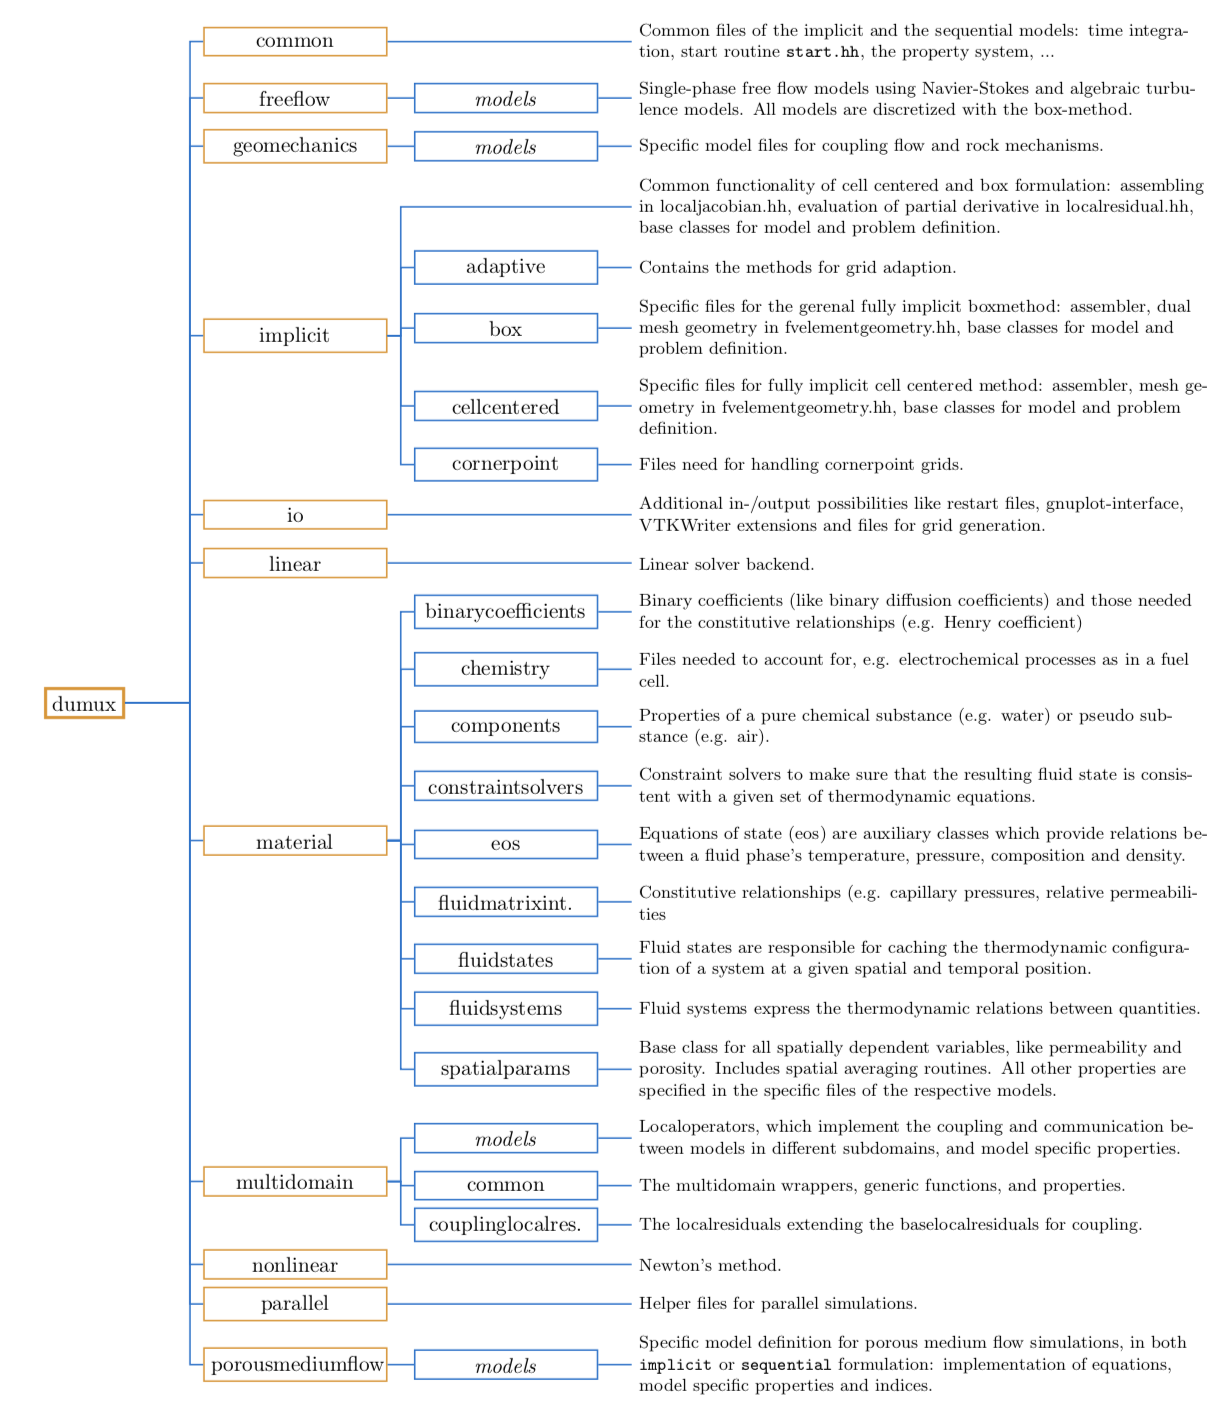
\includegraphics[height=190mm]{dumux_structure}
\caption{\footnotesize The $DuMu^x$ Structure}
\label{fig:dumux_structure}
\end{figure}

\newpage
\subsubsection*{Available Numerical Models}
%What solvers can we use ?
%What can DuMuX offer ?
%List all the models here and explain briefly what can be done, and for what kind of problems this can be used.

As I mentioned, $DuMu^x$ offers a large variety of models that can be used to solve a specific problem. This provides large flexibility in terms of computational cost and stability questions as explained by $DuMu^x$ developers Flemisch et al. \cite{flemischdumux}, \cite{flemisch2007dumux}.
\\One has to take care to choose a solver that is compatible with the given problem. To develop a better feeling for this, the test cases can be studied in detail. A good overview to the user will be given when checking which solver, grid-creator or discretization is used for each type of problem.
\\Nevertheless, using my personal experience, I can say that some information is hard extract, and the incompatibility of some modular pieces inside the $DUNE$ modules, like for example grid creators, can be the cause for some serious errors which were hard to understand and debug without a deep understanding of $DuMu^x$, which again takes time to aquire.
\\I will briefly present some of the numerical models that can be used with $DuMu^x$, so that the reader can later get a better understanding of the model I worked on.\\
\\In $DuMu^x$ there are two types of numerical models: \emph{coupled fully-implicit} and \emph{decoupled semi-implicit}. The difference lies simply in the fact that the so called \emph{coupled fully-implicit} models are strongly modularized, and the user can build a model only prescribing physical quantities like fluxes and source terms. For the \emph{decoupled semi-implicit} models, the user has to work with the actual physical equations, as for example the implementation of the transport equation. As I mainly used the 1p-model to build by oxygen transport model, I will shortly explain what this means and give a few other examples.\\
\\1p basically means that the model is computing the flow for a one phase liquid. If the considered liquid is a mixture of two components, one should rather use the 1p2c model, which takes into account one phase (1p) and two components (2c). We can also consider a two phase liquid by using the two phase (2p) model. I will not go into further details concerning this, as it is rather irrelevant for oxygen computations, but still would like to mention the fact that thermal effects can also be taken into account for most of these models.
\\A more interesting point for us is that some models, as for example the 1p model, can be computed in two separate problem-files describing two flow problems in different networks, and can then be coupled to produce a 1p-1p model computing results in an embedded network. In other words, this coupled model of two separate 1p models can be calculated together, to obtain the pressure in a vessel network, and the pressure in the tissue surrounding this network. This will be explained in more detail in the next section.
\\Further general details concerning $DuMu^x$ and its structure can be found in the $DuMu^x$ reviews  \cite{flemischdumux}, \cite{flemisch2007dumux}.

\subsubsection{Implemented Model}
%Explain what I tried to do.

As mentioned previously, some of the existing test cases can be combined to solve a more sophisticated and specific problem. In our case, this refers to the coupling of the existing tracer model to the 1p-1p model.\\

\subsubsection*{The 1p-1p Model}
%Briefly explain the 1p_1p Model
%Explain how tissue and bloodflow are coupled
%Maybe put some results of the 1p_1p Model here

As I indicated, the 1p-1p model itself is the coupled version of a 1p simulation in a network, and a 1p simulation in the tissue surrounding it. It can simulate the flow of a solute in a network by convection and the diffusion of this solute into the tissue through the coupling. This coupled model was already a very useful tool, and helped me to compute pressure drops in interesting vascular networks as for example glomeruli. The computed pressures seemed physically correct, whereas the velocities seemed rather unrealistic. I will come back to presenting and discussing these results in the Results section \ref{Results}.\\
My main idea was to use the computed velocities from the 1p-1p model, and feed the tracer with this as an input in order to obtain the oxygen transport and diffusion into the tissue and finally get the oxygen field in the tissue for steady-state conditions.\\

%\subsubsection*{\footnotesize 1p-1p Model Impressions}

%Figure \ref{fig:glom2_pressure}  is the result of a $DuMu^x$ blood flow simulation computed on a glomerulus network. The pressure field in the network is visualized.\\
%\begin{figure}[h]
%\centering{
%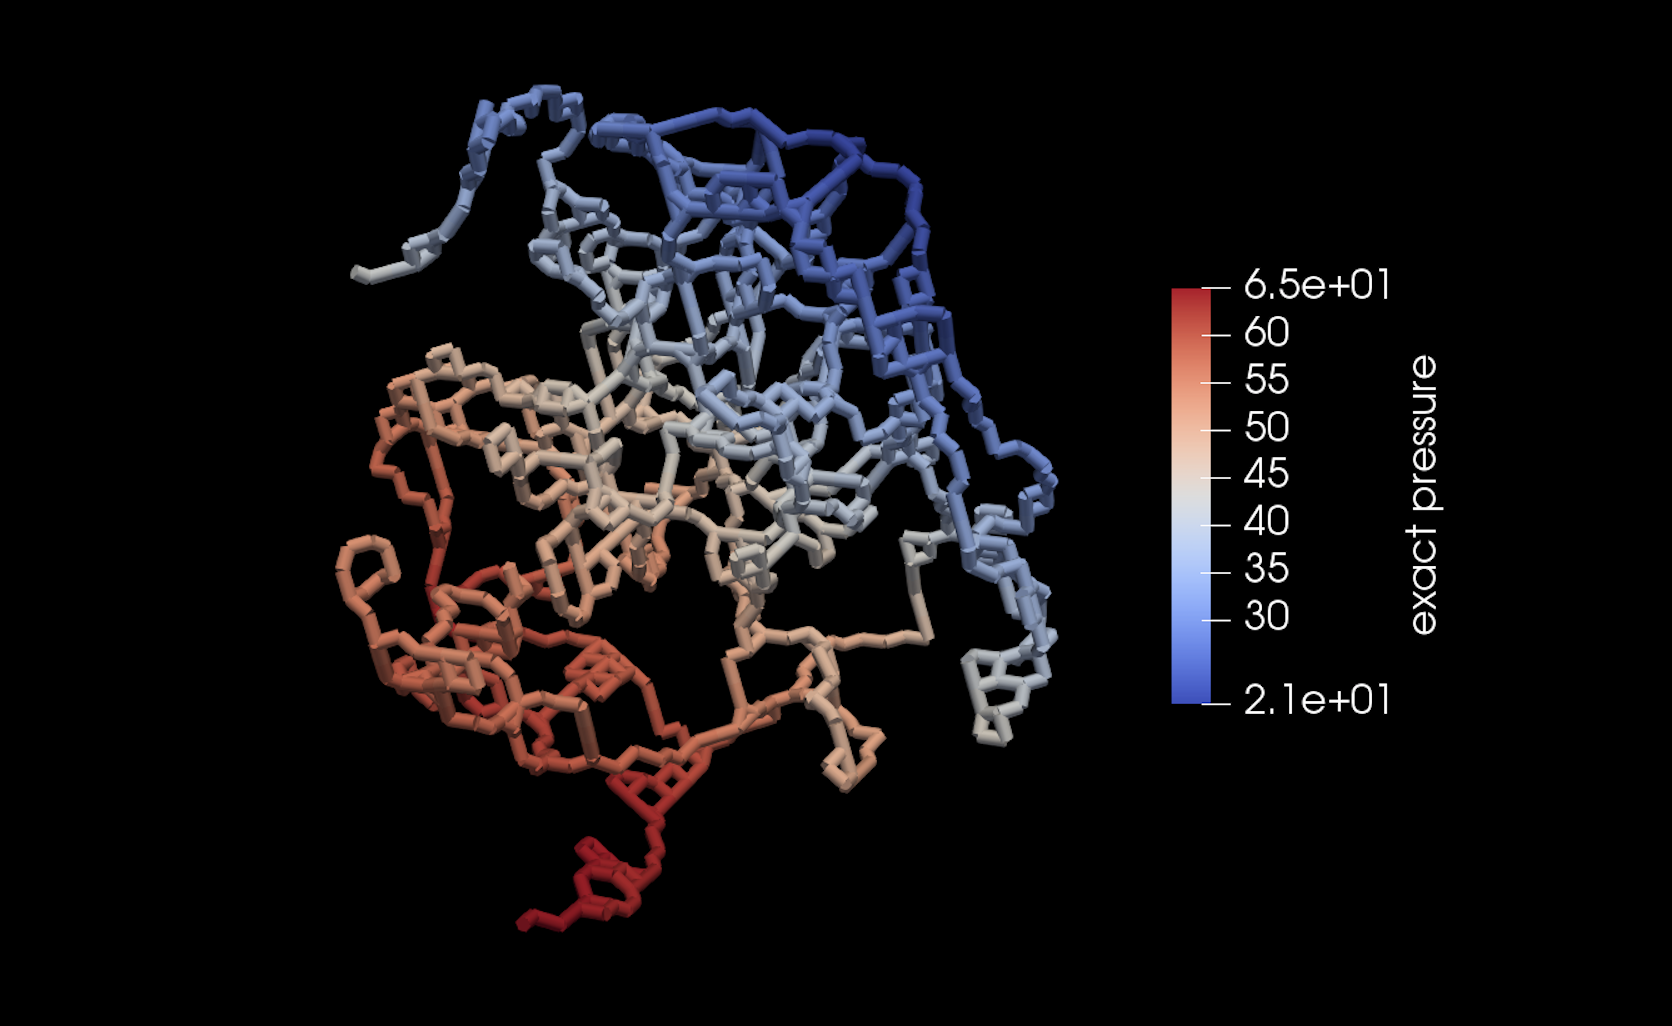
\includegraphics[width=162mm]{glom2_pressure}}
%\caption{\footnotesize $DuMu^x$ Pressure Computations for Glomerulus Network}
%\label{fig:glom2_pressure}
%\end{figure}\\
%
%\\Figure \ref{fig:glom2_velocity}  is the result of a $DuMu^x$ blood flow simulation computed on a glomerulus network. The velocity field in the network is visualized.\\
%\begin{figure}[h]
%\centering{
%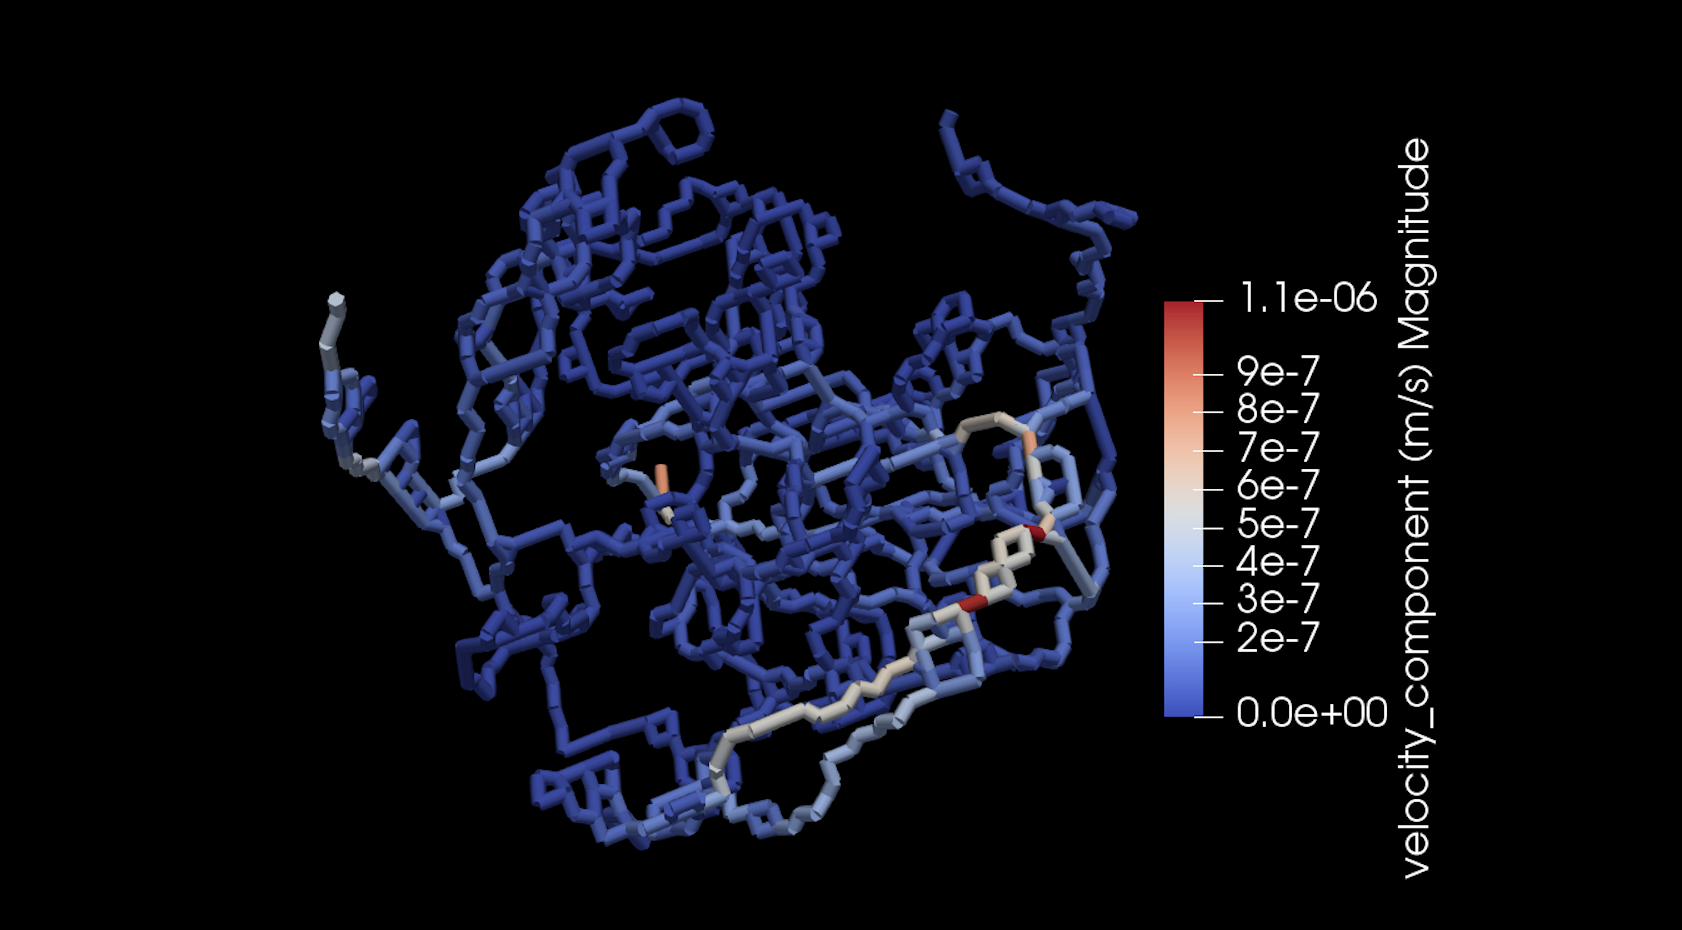
\includegraphics[width=162mm]{glom2_velocity}}
%\caption{\footnotesize $DuMu^x$ Velocity Computations for Glomerulus Network}
%\label{fig:glom2_velocity}
%\end{figure}\\\\

\subsubsection*{The Tracer Model}
%Briefly explain the Tracer Model
%Maybe put some results of the Tracer Model here

The second model I used to build my oxygen tracking model is the tracer. The tracer model can literally \emph{trace} the path of a solute when fluxes or velocities are given as input data. My main idea was to use the computed velocities from the 1p-1p model, and feed the tracer with this as an input in order to obtain the oxygen transport and diffusion into the tissue and finally get the oxygen field in the tissue for steady-state conditions.
\\Generally, the tracer model is computing the distribution of a solute inside a control volume for every time step.
\\As it can \emph{trace} substances in networks of different geometries, and accordingly compute concentrations and concentration fields of solutes in dynamic systems, it seemed like a very interesting option in order to compute the oxygen field in the tissue surrounding a given network.
\\Even though it is hard to show the outputs of the tracer model, a visualization for the first and last time of a tracing simulation is pictured in the Appendix \ref{Tracer}.\\

\newpage
\subsubsection*{The Coupled Model}
%Briefly explain what coupling is and how code is supposed to work
%Hopefully put some results of the coupled model here or explain why the results are wrong

To achieve the goal of tracing oxygen in the given vessel-networks, I coupled the previously described models to obtain a 1p-1p-tracer model.\\
\\I would like to repeat that the velocity output of my previous 1p-1p model is the input for the tracer model. This is important, as I will later explain the problems I had when trying to produce results with this model. Generally I wanted to get the concentration of my solute of interest, which is oxygen, for every time step.
\\As my goal was to compute oxygen fields not only in the network, but also in the tissue surrounding it, I had to create a 1p-1p-tracer-tracer model. The second tracer is coupled in order to compute the oxygen concentration not only in the vessels (this is what a 1p-1p-tracer model would do) but also for the tissue. Due to time limitations, the implementation of this model did not complete fully and is left for future efforts. Further explanations concerning this will follow in the Results \ref{Results} section.

%%%%%%%%%%%%%%%%%%%%%%%%%%%%%%%%%%%%%%%%%%%%%%%%%%
\newpage
\section{Simulation Results and Analysis}
\label{Results}
%Put all the results here - Should be easier to understand things
In this section, the produced results using the two introduced methods will be presented and analyzed for a few different networks. Finally the results will be discussed and the methods will be compared. The accuracy of produced results as well as the physiological meaning behind these results will be the main subject in this chapter.

\subsection{Results of the Green's Function Method}
\label{ResultsGreens}
%Main part of the Thesis
%Results part of Green's
%-Present some results on different networks
%- Plots and Results (maybe 3 I already have + 2 new ones)
%-Explanation of plots
%-Explaining inputs/outputs and meanings is in Appendix

The Green's Function Method is providing many outputs which are specified in more detail in the Appendix \ref{Outputs}. In this section, some of these outputs will be presented and explained. The physiological meaning will be described and finally the results will be discussed.

\subsubsection*{Krogh Model as an Introduction}
\label{Krogh}
%Explain relevance of this model and the produced results (many plots here)

%Present Network
The Krogh model describes the vessels as cylinders and the tissue as concentric cylinders surrounding the vessels. In this model, it is assumed that the capillaries are straight and parallel. The blood flow in all the capillaries is assumed to be unidirectional, and the distribution of capillaries is assumed to be homogeneous \cite{kreuzer1982oxygen}. As one might expect, this model has a few unrealistic assumptions, but as it is a straightforward network, it is the most basic model to start with to validate a computational method.\\
%Explain Plot
\\The Krogh model has been a standard simulation network used as an initial point for developments as it has a very easy and simple structure.
Figure \ref{fig:Contour_Krogh} is the result of a Green's Method blood flow simulation computed on a Krogh network. The Solute Concentration in the network and in the tissue is visualized in the form of a slice (see output section \ref{Outputs} for more information). The illustration shows an impression of oxygen levels in the tissue and the vessel segments, and generally gives the local oxygen concentrations in mmHg.\\\\
\begin{figure}[h]
\centering
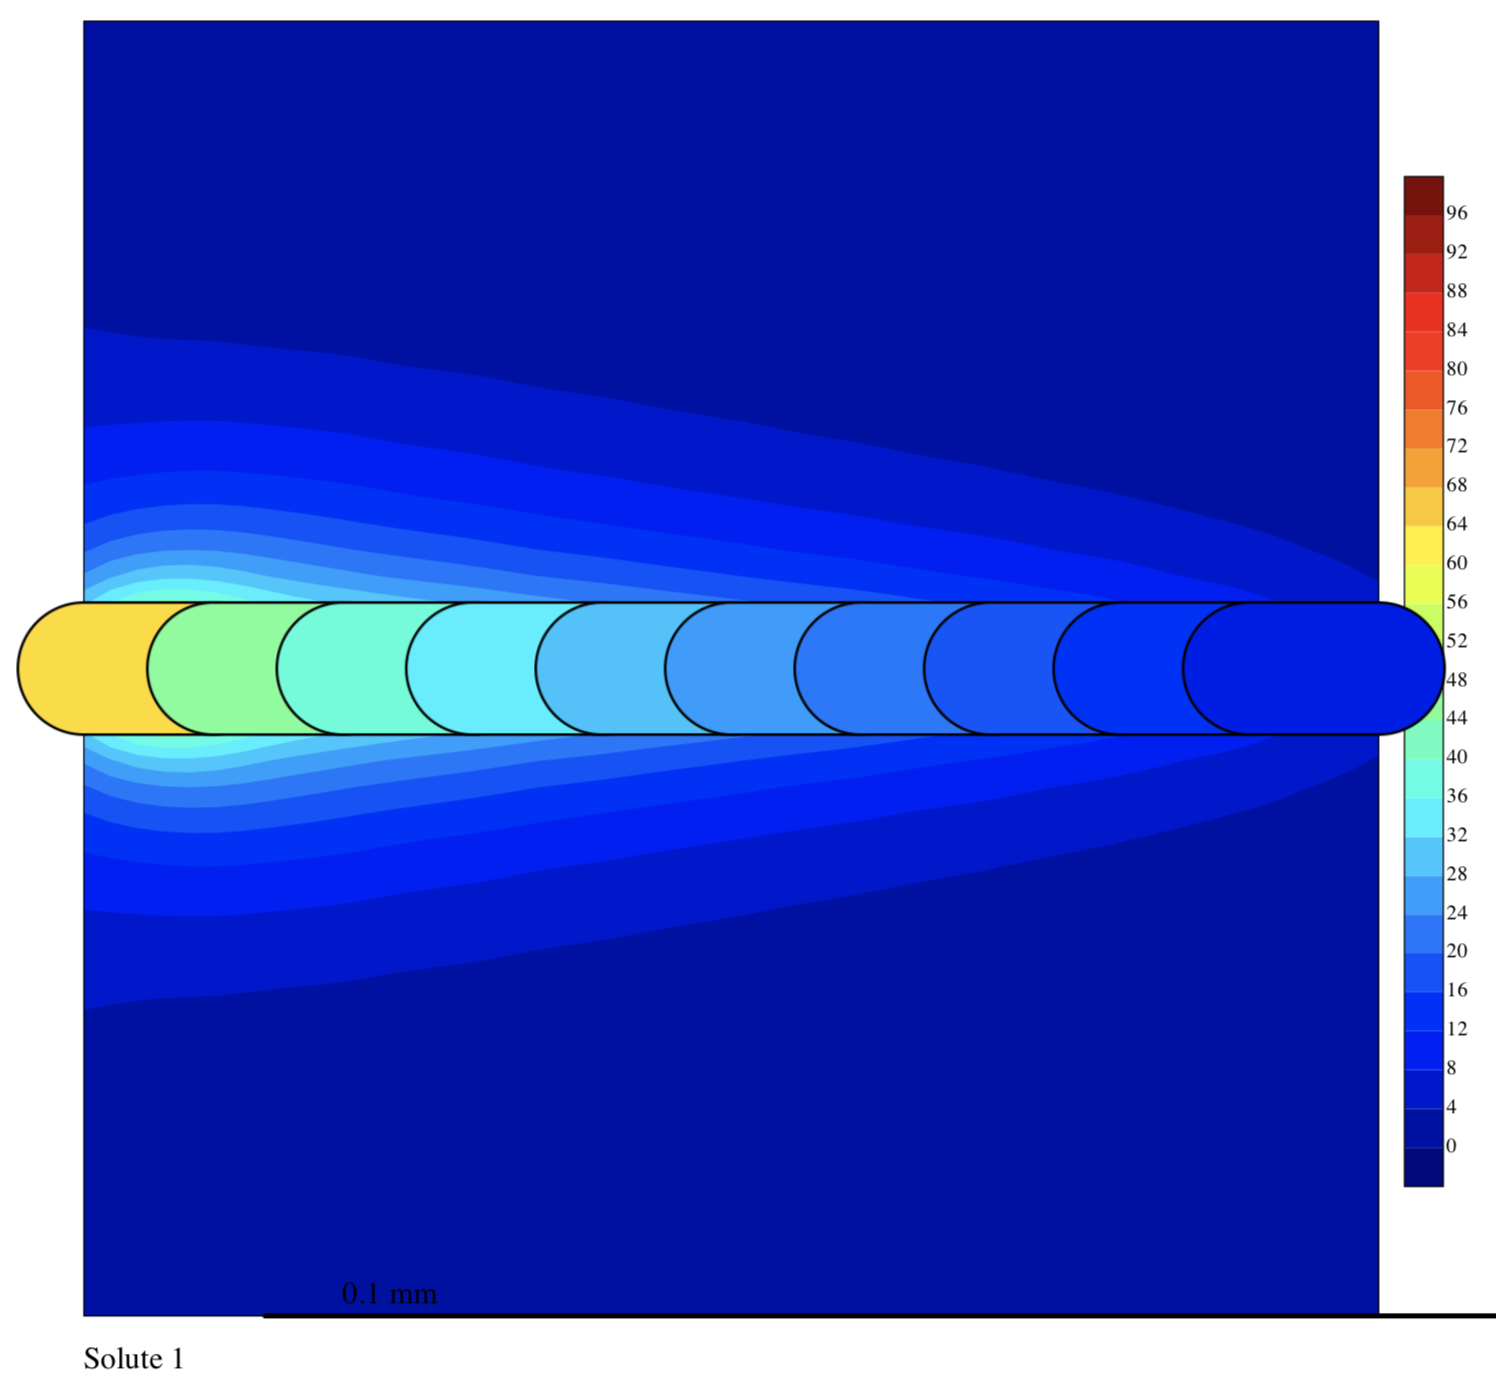
\includegraphics[width=120mm]{Contour_Krogh}
\caption{\footnotesize Green's Contour Output for Krogh Network}
\label{fig:Contour_Krogh}
\end{figure}
%Explain Results
\\One can clearly see that the results produced are physically realistic. In figure \ref{fig:Contour_Krogh}, one can see that the blood flow goes from left to right. The $O_2$ concentration in mmHg accordingly goes down in flow direction. The concentrations as well as the diffusive distance in the tissue also decrease in flow direction, which can be explained by the fact that a lower concentration gradient goes with a lower diffusive flux. This is in accordance with Fick's Law of Diffusion \ref{Fick}. As one can see from the input files \ref{Inputs}, the diffusivity constant $\alpha$ is constant for homogeneous tissue. Due to the fact that the diameter of the vessels is constant as well when considering the Krogh model, the intravascular resistance to radial oxygen transport K for each diameter/vessel is also constant. Differences in diffusive fluxes and oxygen penetration distances into the tissue therefore mainly depend on the $PO_2$ gradients themselves.\\
\\Eventually, one can see that the results computed on the Krogh network show that the Green's function method performs well and produces physically accurate results on simplified and perfectly homogeneous networks as this one.
\\It is further remarked that analytical solutions of the Krogh cylinder model have been derived before and the results shown in this figure correspond well to the  analytical results. This validates that the Green's function method and the corresponding implementation can produce physically accurate results, and suggests that it is a suitable method to conduct further studies.

\newpage
\subsubsection*{A First Tumor Network}
%Explain relevance of this model and the produced results (many plots here)

%Present Network
The Green's function code provided by Prof. Secomb contains a few microvascular networks as examples, which can be studied and extended. In this thesis, I executed many of those models to get a good understanding of physiological phenomena concerning $O_2$ transport in various organs and different networks.
\\Two of these example networks provided by Prof. Secomb are the tumor networks. I will first present the results obtained for the first network, and later get to the more complex and relevant second example.
\\The Tumor 1 network is more complicated than the previously presented Krogh model but generally gives a way better insight to the results than the Cardiac Network simulation, due to the much lower vessel density. The result is visualized on Figure \ref{fig:Contour_Tumor1998}. One can see the result of a Green's method blood flow simulation computed on a simple tumor network. As for the previous network, the oxygen concentration in the network and in the tissue is visualized in the form of a two dimensional slice (see output section \ref{Outputs} for more information). Again the illustration shows an impression of oxygen levels in the tissue and the vessel segments, and generally gives the local oxygen concentrations in mmHg.\\\\
%Explain Plot
The Tumor network provided by Secomb was used for further simulations and to validate the produced data.
Figure \ref{fig:Contour_Tumor1998}  is the result of a Green's method blood flow simulation computed on a tumor network. The solute concentration in the network is visualized.\\
\begin{figure}[h]
\centering
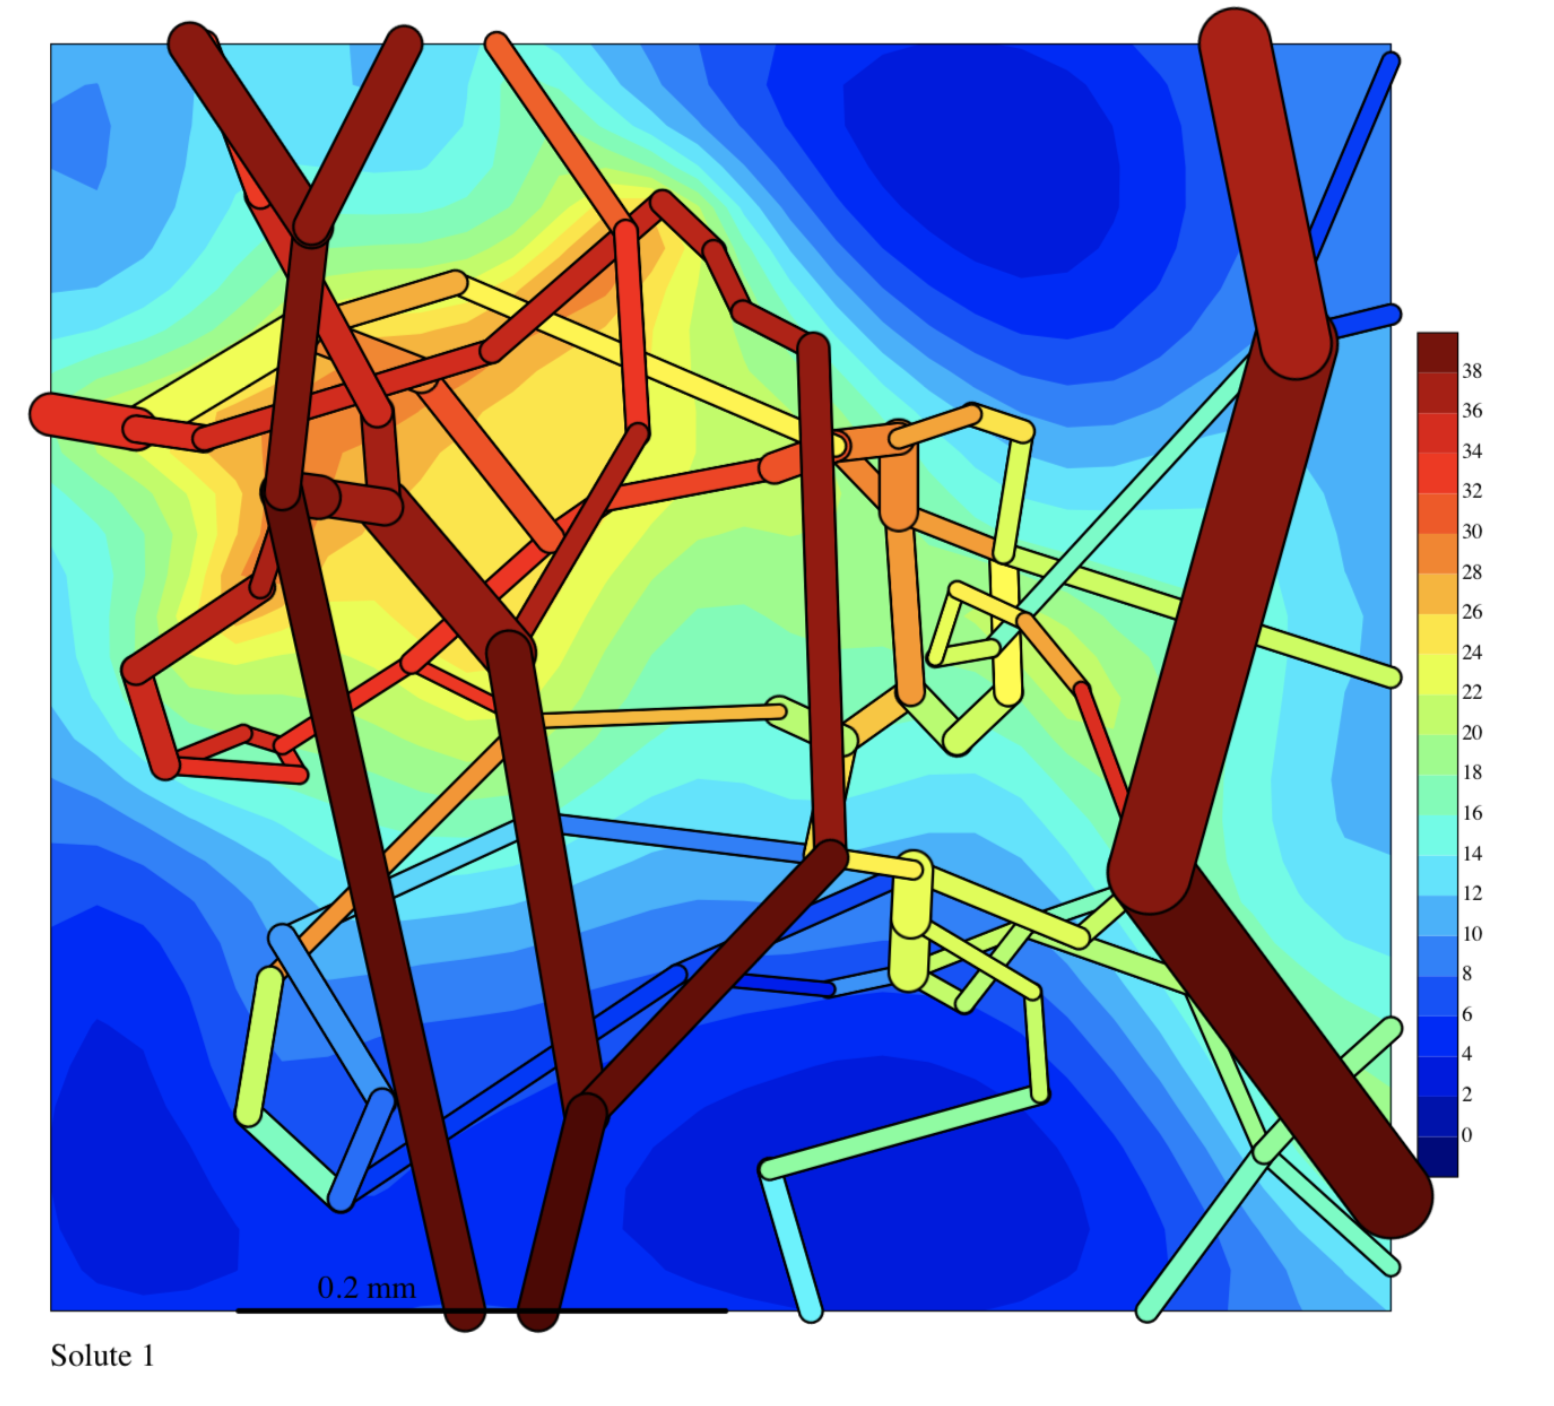
\includegraphics[width=120mm]{Contour_Tumor1998}
\caption{\footnotesize Green's Contour Output for Tumor 1}
\label{fig:Contour_Tumor1998}
\end{figure}\\
%Explain Results
\\As contour-plots generally show a \emph{compressed} picture of a three dimensional network, many vessels that are \emph{above} each other are shown as if they were intersecting. This can be hard to differentiate for the output files of some complex networks. In this case, this tumor network doesn't have many vessels, but is rather supplied by a few thicker vessels. The red color corresponds to oxygen enriched blood, and clearly oxygen in tissue regions proximal to these vessels is higher. We do not have any information about the exact origin of this particular image segmentation, but it can be observed that the length of segments within vessels is quite large. This is a limitation in order to obtain a precise resolution of the computed oxygen field, as $PO_2$ is always computed for each node and segment. Eventually a $PO_2$ value is assigned to each segment. This means that a lower resolution for the oxygen field is obtained.
\\In this case, $PO_2$ levels reach up to about $40$ mmHg which lies within the physiological range.

%\subsubsection*{Brain Model}
%Explain relevance of this model and the produced results (many plots here)

%The Brain network provided by Secomb (?) was used for further simulations and to validate the produced data.

\newpage
\subsubsection*{The Cardiac Network}
%Explain relevance of this model and the produced results (many plots here)
%The Cardiac network provided by Secomb was used for further simulations and to analyze results in more complex networks.\\

%Present Network
Another interesting example network is the cardiac network. Even though we do not have specific informations about how this particular image segmentation was obtained, knowing that it is a cardiac network, one might expect a high density of vessels for this network.
\\In this section, the oxygen distribution in a cardiac network will be presented. This network is more complicated than the previously presented Krogh model \ref{Krogh}. The result is visualized on Figure~\ref{fig:Contour_Cardiac1}. The given output shows the result of a Green's method blood flow simulation computed on a cardiac network. As for the Krogh and the Tumor 1 networks, the oxygen concentration in the network and in the tissue is visualized in the form of a slice (see output section \ref{Outputs} for more information). Again the illustration shows an impression of oxygen levels in the tissue and the vessel segments, and generally gives the local oxygen concentrations in mmHg.\\
%Explain Plot
\begin{figure}[h]
\centering
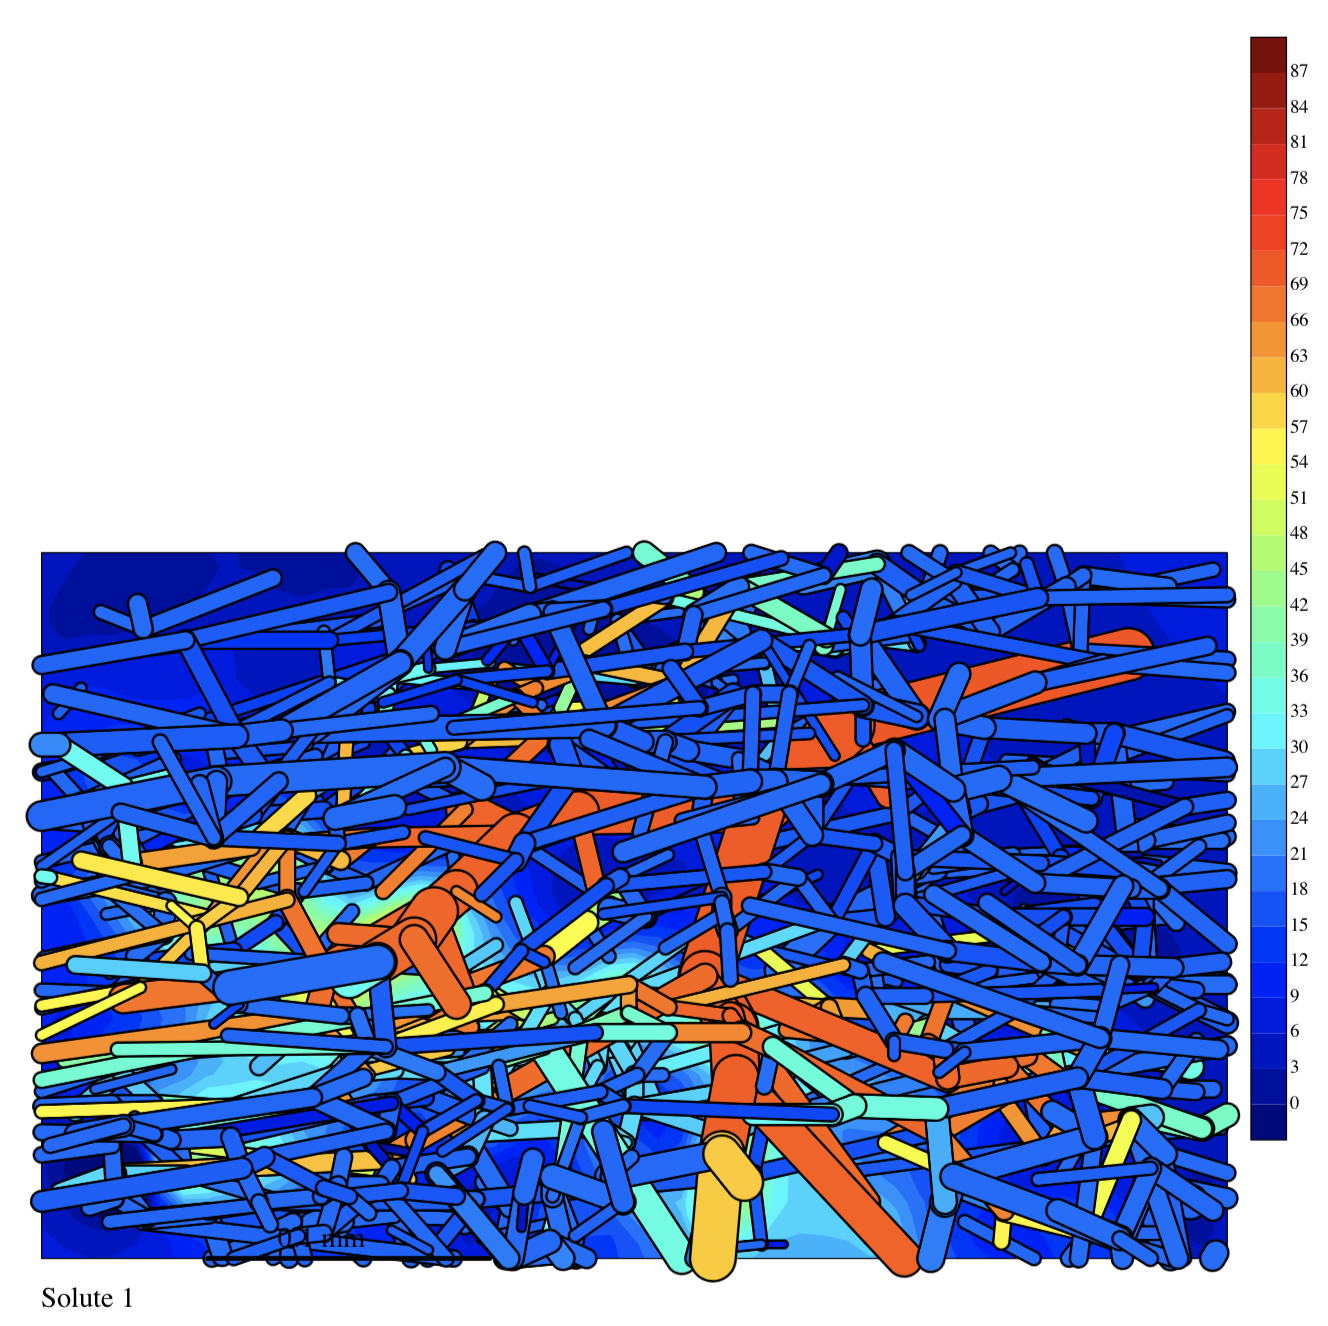
\includegraphics[width=120mm]{Contour_Cardiac}
\caption{\footnotesize Green's Contour Output for Cardiac Network}
\label{fig:Contour_Cardiac1}
\end{figure}
\\Figure~\ref{fig:Contour_Cardiac1} shows the distribution of oxygen in a small
network of vessels.
%Explain Results
The three dimensional network of vessels is \emph{compressed} to a two
dimensional representation in order to get a simpler output file. This kind of output has the advantage of encapsulating most of the computed values, even though it might look complex for some networks, where the oxygen fields are very heterogeneous. The red color corresponds to oxygen enriched blood. The principle vessels go through the middle of the three dimensional tissue section and therefore have the highest oxygen partial pressures which are around $65$ mmHg. The oxygen concentration in the finer and smaller vessels surrounding the big oxygen-supplying vessels accordingly decreases with growing distance from the oxygen sources.
But still the oxygen in tissue regions proximal to the bigger oxygen-supplying vessels is higher. Once again, it can be observed that the length of segments within vessels is quite large, which causes a lower oxygen field resolution.
\\The $PO_2$ levels reach up to about $84$ mmHg within a physiological range.

\newpage
\subsubsection*{The Mesenteric Artery Network}
\label{Mesent}
%Explain relevance of this model and the produced results (many plots here)
%The Mesenteric Artery network provided by Secomb was used for further simulations and to get more computational results.\\

%Present Network
Another example network provided by Prof. Secomb is the mesenteric artery network.
\\Like for the previously presented networks, we don't have specific information concerning the network. In the absence of information, this network is used as a sample network to study the computational results. Knowing that it is supposed to represent a mesenteric artery network, which is an artery supplying the large intestine, one can clearly see the very small vessels surrounding the main arterial tree. These vessels are embedded in the intestine itself and supply oxygen to the surrounding cells.
\\Generally the vessels are very fine and the vessel resolution is high, which entails a good oxygen field resolution for the tissue surrounding the vessels.
\\The result is visualized on Figure \ref{fig:Contour_Mesent1}. The output shows the result of a Green's method blood flow simulation computed on a mesenteric artery network. As for the previous networks, the oxygen concentration in the network and in the tissue is visualized in the form of a slice (see output section \ref{Outputs} for more information). Again the illustration shows an impression of oxygen levels in the tissue and the vessel segments, and generally gives the local oxygen concentrations in mmHg.
%Explain Plot
\begin{figure}[h]
\centering
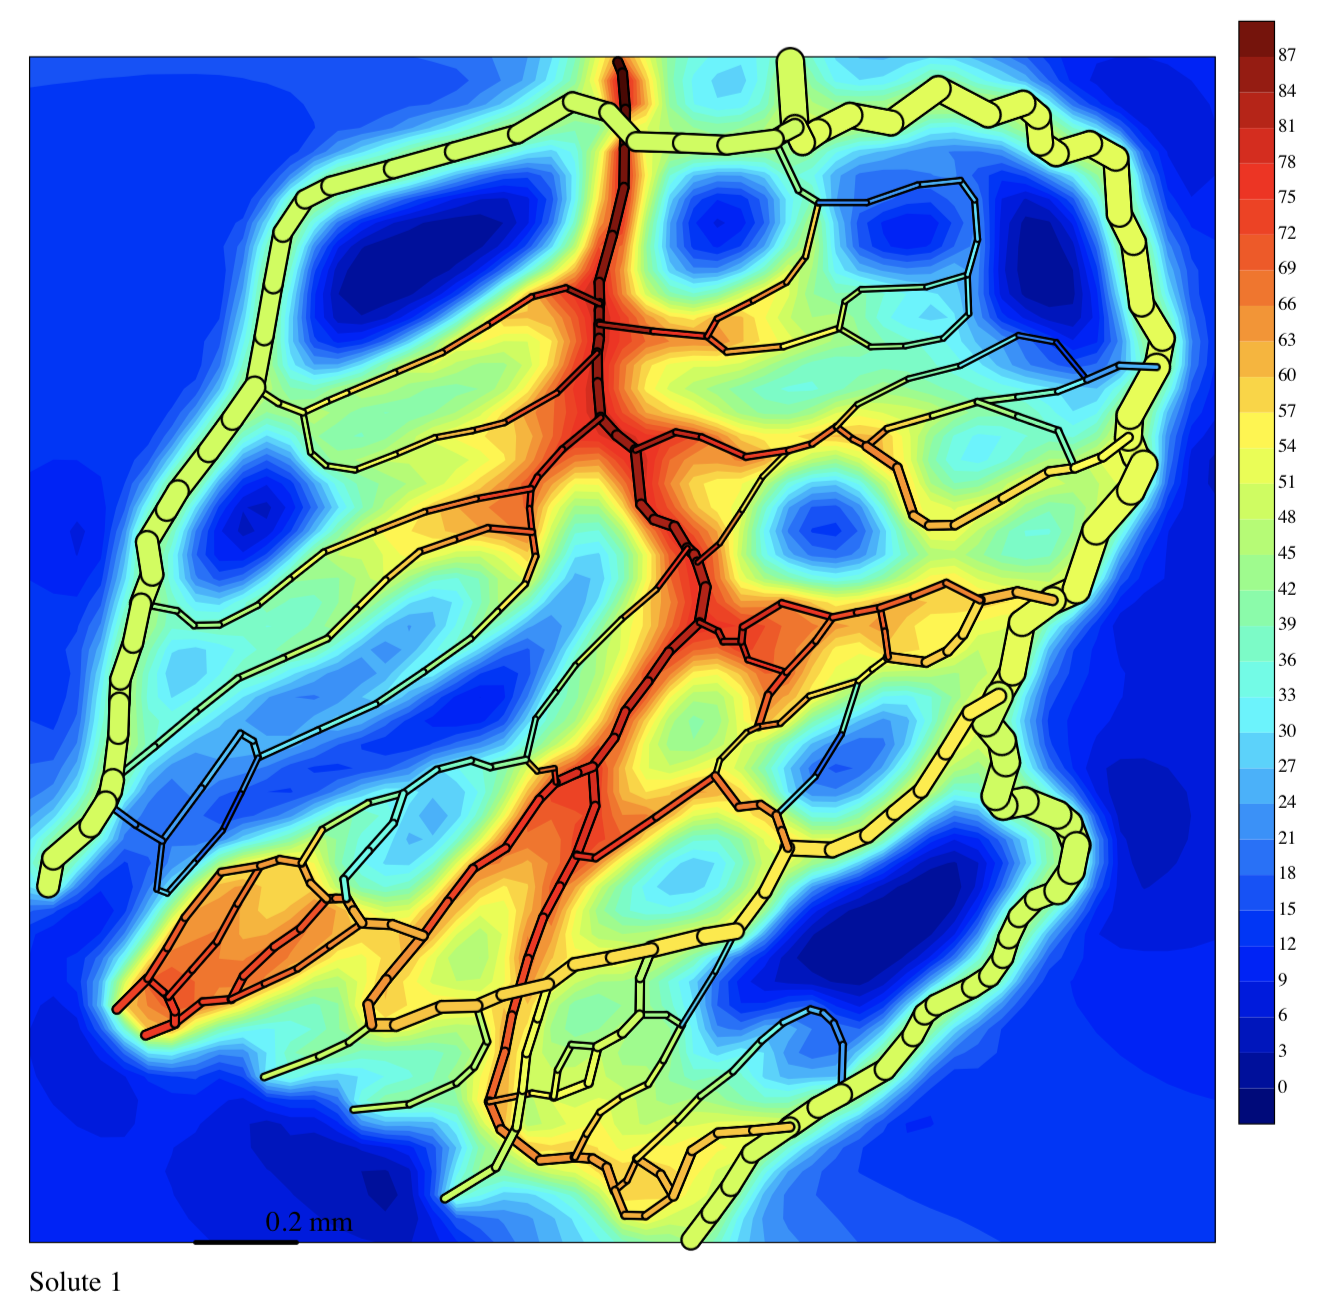
\includegraphics[width=120mm]{Contour_Mesent1}
\caption{\footnotesize Green's Contour Output for a Mesenteric Artery Network (Solute 1)}
\label{fig:Contour_Mesent1}
\end{figure}
%
%\\Figure \ref{fig:Contour_Mesent2}  is the result of a Green's Method blood flow simulation computed on a Mesenteric Artery network. The Solute Concentration of Solute 2 in the network is visualized.\\
%\begin{figure}[h]
%\centering
%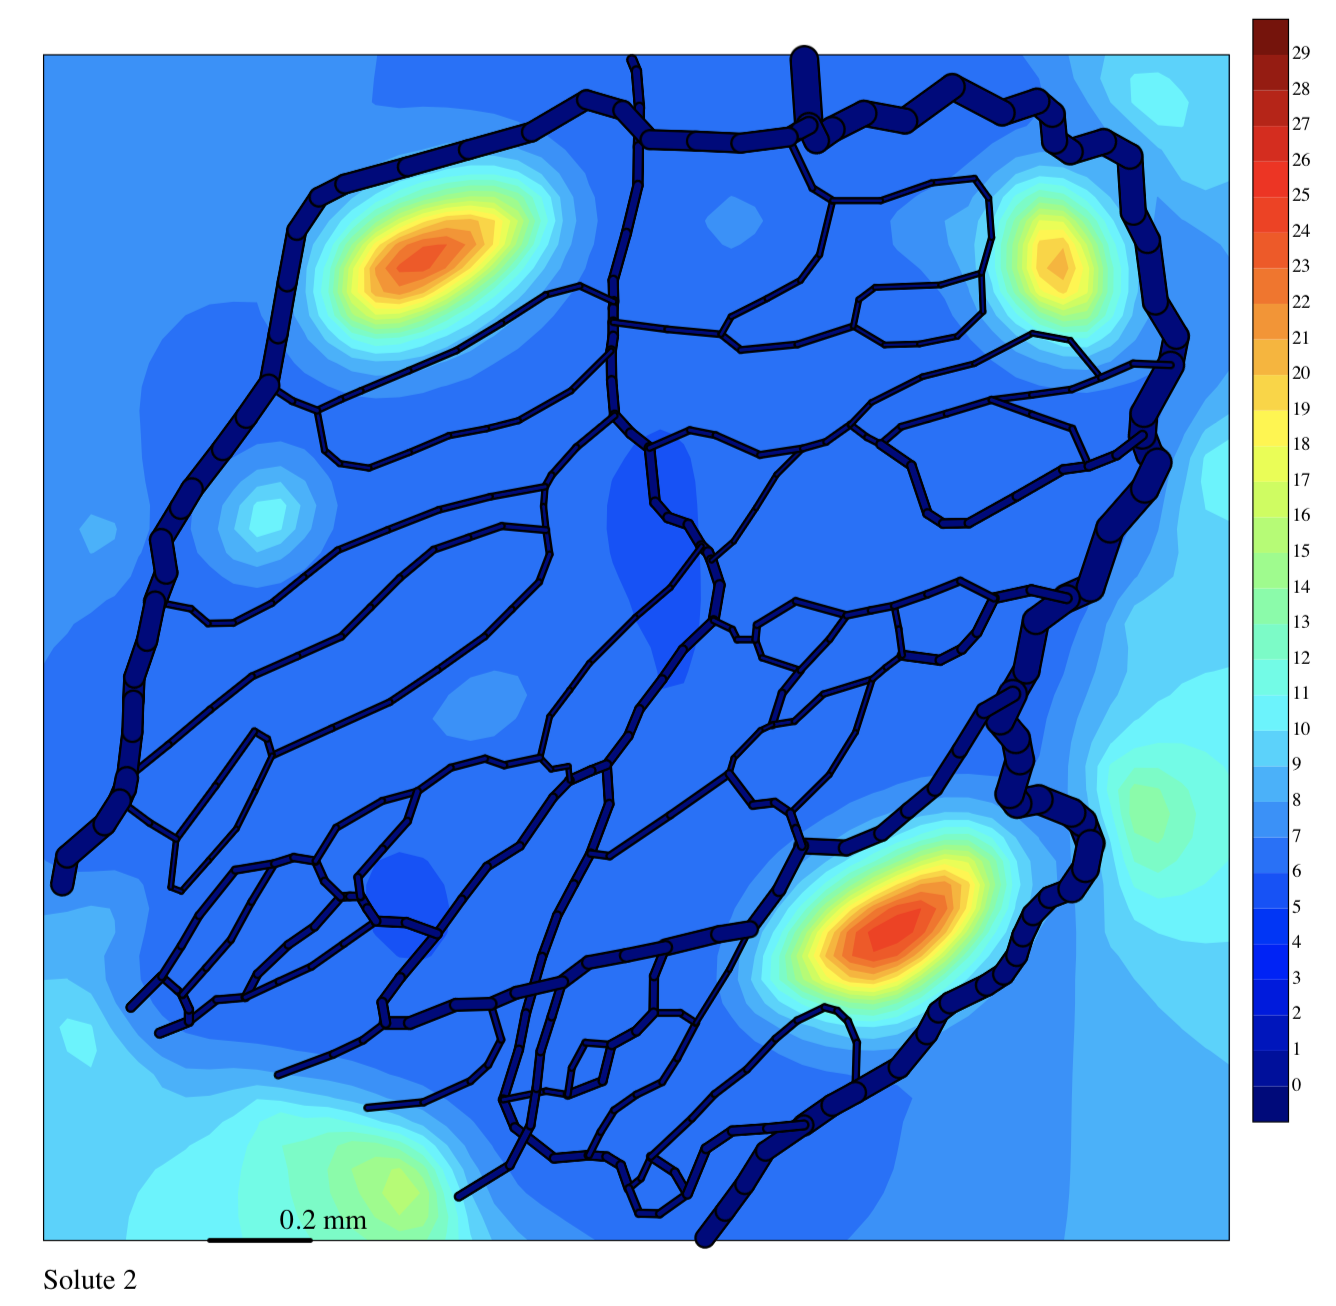
\includegraphics[width=85mm]{Contour_Mesent2}
%\caption{\footnotesize Green's Contour Output for a Mesenteric Artery Network (Solute 2)}
%\label{fig:Contour_Mesent2}
%\end{figure}
\\
%Explain Results
\\This network is more complicated than the previously presented networks but generally gives a better insight to the results than the cardiac network simulation, due to the much lower vessel density. Especially the tissue concentrations and the changing oxygen concentrations in longitudinal direction of the vessels can be seen very well.
\\Due to the low density of capillaries for this network, this figure can give a good insight to the values computed by the Green's model code. One can clearly see that the partial pressure of $O_2$ goes down in radial direction with growing distance from the vessels. At hotspots where the capillary density is higher due to branching and ramification, the diffusion comes from two vessels and the superposition of two close source elements leads to peaks in $PO_2$ values.\\
\\From a physiological point of view, the computational result is correct when assuming that the oxygen consumption through the whole intestine is constant. The oxygen supply to the intestinal vessels surrounding the main arterial tree is constant, and the oxygen concentrations in the intestinal ares are slightly above 50 mmHg, which is in the physiological range.
\\The general oxygen field clearly shows that some hypoxic regions can be found at spots without vessels or where the vessels themselves have a very low $PO_2$ concentration. With $PO_2$ values ranging from $0$ mmHg (hypoxic region) to 87 mmHg, the results for the whole sample lie once more in the physiological range.

\newpage
\subsubsection*{A Second Tumor Network}
\label{Tumor}
%Explain relevance of this model and the produced results (many plots here)

%Present Network
Another interesting tumor example network provided by Prof. Secomb is the Tumor 2 network.
\\Even though there is no information given about how this particular image segmentation was obtained, knowing that it is a tumor network, one might expect a random ramification and distribution of vessels. In fact, this network is build by vessels of different sizes and the oxygen concentrations within the vessels is largely varying.
\\The Tumor 2 network is more complicated than the previously presented Tumor 1 network and the computational simulation produces a very interesting output. The result is visualized on Figure \ref{fig:Contour_TumorDuke}. Here one can see the result of a Green's Method blood flow simulation computed on a simple Tumor network. As for the previous models, the Oxygen Concentration in the network and in the tissue is visualized in the form of a slice (see output section \ref{Outputs} for more information). Again the illustration shows a virtual cut into the tissue and gives local oxygen concentrations in mmHg.\\\\
%Explain Plot
Figure \ref{fig:Contour_TumorDuke}  is the result of a Green's method blood flow simulation computed on a tumor network. The oxygen concentration in the network and the tissue is visualized.\\
\begin{figure}[h]
\centering
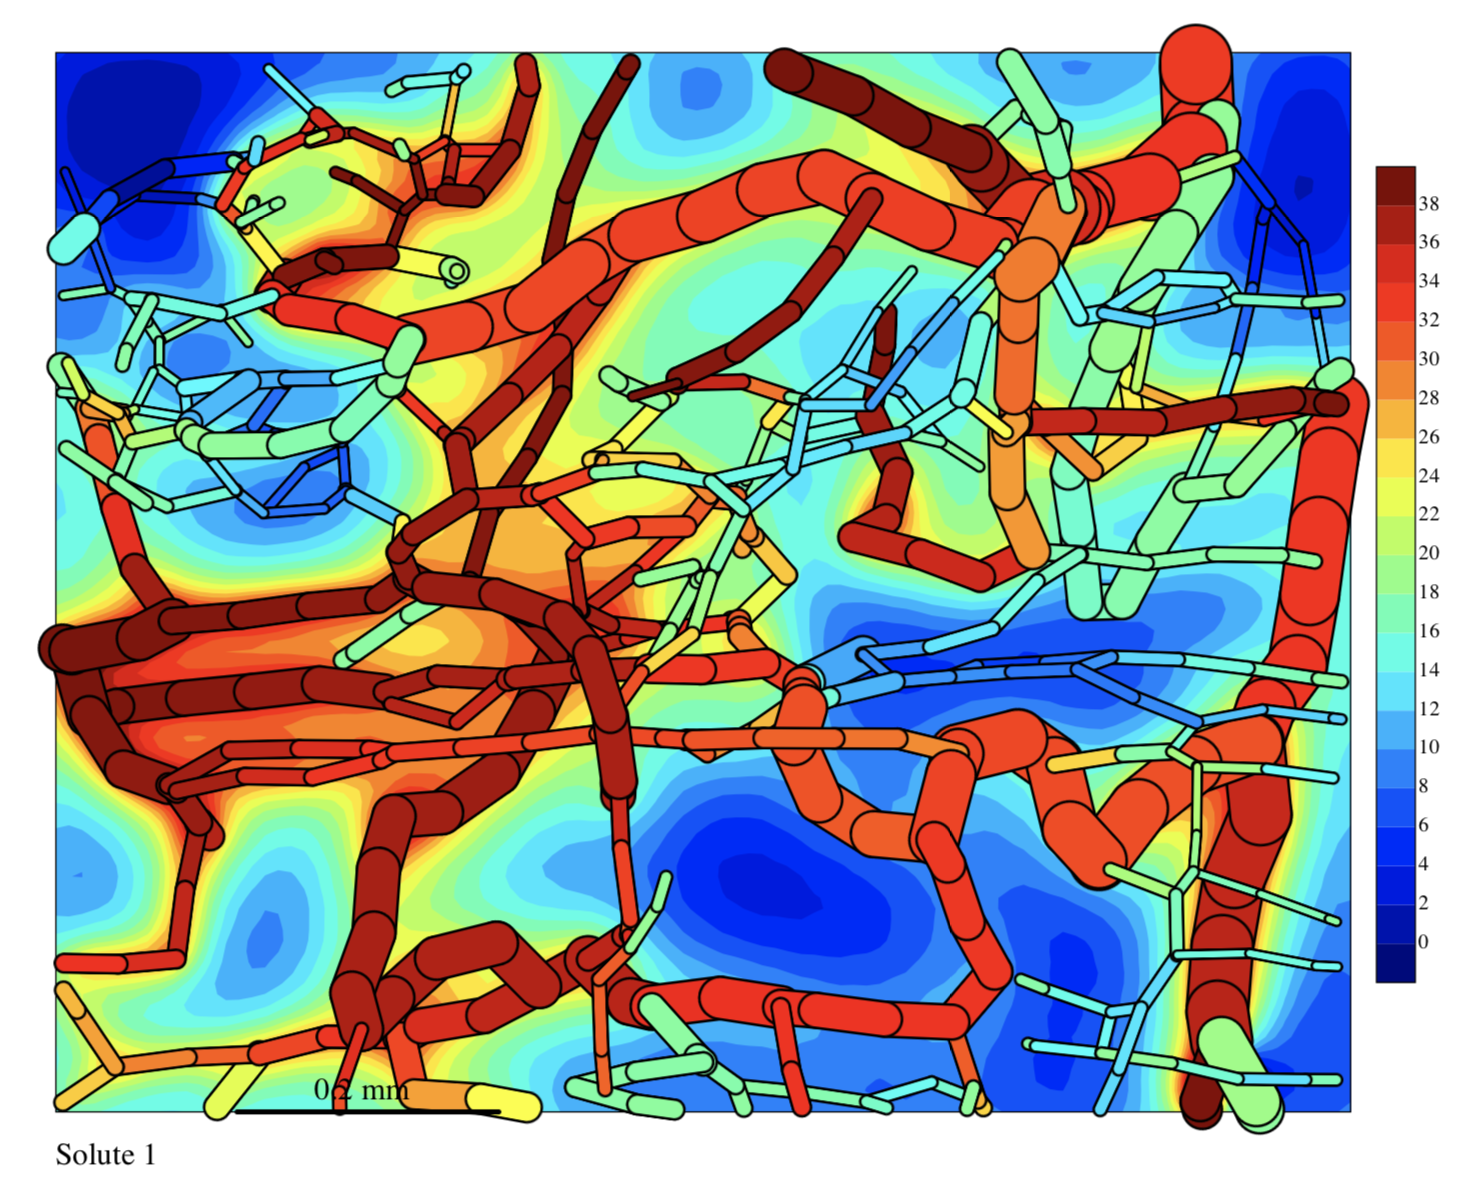
\includegraphics[width=120mm]{Contour_TumorDuke}
\caption{\footnotesize Green's Contour Output for Tumor 2}
\label{fig:Contour_TumorDuke}
\end{figure}\\
%Explain Results
\\The overlapping of the vessels with different oxygen concentrations is due to the fact that the three dimensional space of vessels is projected on a two dimensional plane, as for the previous examples. The red color corresponds to oxygen enriched blood which is in this case carried by the thicker vessels supplying this sample of tissue. The oxygen partial pressure in the tissue regions proximal to these bigger vessels is higher with peaks around $40$ mmHg. The segmentation resolution depends on the vessel, but is overall rather high, which entails a high resolution for the oxygen field in the tissue.
\\Generally the highest $PO_2$ levels can be found surrounding the big vessels and especially in regions where many sources are overlapping. This is due to the fact that the source terms are superpositioned when calculating the oxygen field during the computational iterations, and makes sense from a physiological point of view, as a lot of oxygen is supplied to these areas.
\\The $PO_2$ levels range between around $3$ and $40$ mmHg within a physiological range. Generally the average $PO_2$ in this sample is quite high, due to the equally distributed and well oxygenated big vessels.

\newpage
\subsubsection*{Further Outlook for New Networks}
\label{Outlook}
%Explain relevance of the new models and the produced results (many plots here)
%These results are wrong !!! why ?
%In this section the goal is to see how this method can perform in general when it is applied to new networks and to discuss the produced results in detail.

An overview to simulation results of the Green's method was presented for different networks. The networks covered a range from homogeneous and simple vasculatures to rather complex and heterogeneous samples. Some of the examples were physiologically very interesting as were the computed oxygen fields within the tissue.
\\Considering how well this method seems to perform for some complex networks I presented in the last section, the question of how well it can perform for new networks obtained through imaging techniques was raised. For this reason, I tried to simulate the oxygen field on a glomerulus network using the Green's method code. The same glomerulus network was also used for $DuMu^x$ simulations (Glomerulus 1, Figure \ref{fig:glom_pressure}).\\
\\In general, computing oxygen fields with diffusion into the tissue is physiologically meaningless for a glomerular network, as in reality glomeruli are not surrounded by normal tissue. In this case, I considered the glomerular network as a vascular network example, and used it as a simple vasculature, as if the network was embedded anywhere else in homogeneous tissue.
\\Figure \ref{fig:NetNodesSegs_Glom} is one of the ouputs of a Green's method oxygen field simulation computed on a glomerulus network. In this case, the presented output file is not a contour plot, but rather a plot illustrating the labeled nodes and vessel segments in the given network. This type of plot is called \emph{NedNodesSegs} and is supposed to give an overview of the used segments and nodes in the network.
\\At this point, I would like to mention that the code did not run as expected, and thus didn't produce a sink field. As the Green's method iteratively computes a source and a sink field, which are used to obtain the oxygen distribution field by superposition, no oxygen field could be computed. The numbers written on the output file \ref{fig:NetNodesSegs_Glom} are the numerations of the segments and the nodes, which was successfully done by the code (see output section \ref{Outputs} for more information).
\\This shows that this very complex network, which is the Glomerulus 1 network, could be fully recognized, which is already an interesting achievement. However, no computations in terms of oxygen fields could be made, neither in vessels, nor in the virtual tissue (again real glomeruli are not surrounded by tissue). The reasons for this could not be investigated in detail due to time restrictions, and will remain a task for future research. As the network is very complex, for now no correct explanation can be given without doubts. It is likely that there might be a problem with the parameters we chose concerning the solute or the intravascular resistance (see Input Section \ref{Inputs} for more information).

\newpage
\subsection{Discussion of the Green's Method and the Produced Results}
\label{DiscGreens}
%Discussion part of Green's
%Final thoughts about Green's Method for physiological applications and oxygen delivery simulations/computations.
%Compare the results with physiological measured values and check if the results make sense in general.

As the presented examples show, the Green's method and its implementation can produce some excellent results in terms of oxygen field simulations in networks.\\
\\The results are in accord with the previously presented physical laws, which describe the oxygen transport from the vessel to the tissue. Moreover, the results are physiologically accurate. The computed values generally range between $0$ mmHg (hypoxic tissue) and $87$ mmHg (well oxygenated tissue) and seem to be in the physiological range.
\\Even though these computations have been made on networks that were derived from organs, no information was given about how the particular image segmentations were obtained. This also makes it hard to compare the results with experimental values, especially as we don't have physiological data available for these specific networks. In particular, I want to point out that the computed values cannot be compared to any specific values that we could expect or that were previously measured in the past. We can only say that the values are generally in the physiological range and that the physical properties of oxygen transport and diffusion are well respected and in accord with the simulation results, as we don't know anything in particular about the provenance of the networks.\\
\\Particularly interesting results could be observed for the mesenteric artery network and the second tumor example, as the contour plots for these networks provided a vey good insight to the computed oxygen fields inside the tissue and around the vessels. Being able to compute oxygen fields for complex three dimensional networks on this level underlines the qualities of the used method and its ability to perform computations on complex vasculatures.\\
\\However, using the glomerulus network in the last section \ref{Outlook}, we have seen that the Green's method cannot directly compute an oxygen field for any arbitrary vasculature. The reasons for this are not clear yet and will have to be understood in the future, but it seems like the parameters specified for each network have to be tuned in order to produce the expected oxygen fields. The network data given to the code as an input was in the same form as the previous input files, but still might be an error source that couldn't be resolved. Other possible error sources might be in the values given in the other input files (see \ref{Inputs} for more information about the input files). While the code was running, it seemed like the first guess for the oxygen source field and accordingly for the oxygen sink field couldn't be made, and thus the following iterations couldn't compute an oxygen field.
\\For a deeper understanding of the performance of this method, further research has to be made using new networks. It would make sense to use networks for which the provenance is known, as for the presented glomerulus.

\newpage
\subsection{Results of $DuMu^x$} 
\label{ResultsDum}
%Interesting but shorter part, due to the fact that DuMuX is not really producing anything yet
%Results part of DuMuX
%-Pros/Cons
%\\-Quality of results
%\\-Paraview Visualization of results

Some blood flow simulations were run to evaluate the quality of results that can be produced using $DuMu^x$ \ref{$DuMu^x$}. In this section I will present and explain some results produced by $DuMu^x$, and some rather physical than physiological interpretations of simulation results will be discussed. The results of the previously presented 1p-1p model will be shown, and some details about the implemented 1p-1p-tracer model will be given at the end.

\subsubsection*{Some Glomerulus Network Simulations}
%I will hopefully put 1p_1p_tracer results here later
%Discuss the pressure drop from afferent to efferent vessel/arteriol
%Explain some physical things behind it and be creative

In order to analyze the pressure differences and the pressure drop through a glomerulus network, the 1p-1p model was run on several different glomeruli. Coming from an engineering background, pressure variations and drops in simple pipes was a topic I had worked with. However complex networks like the ones that can be found in glomeruli were nothing I had seen until now, and the explanation behind the pressure distribution inside the glomerulus is quite an unknown field.\\
\begin{figure}[h]
\centering
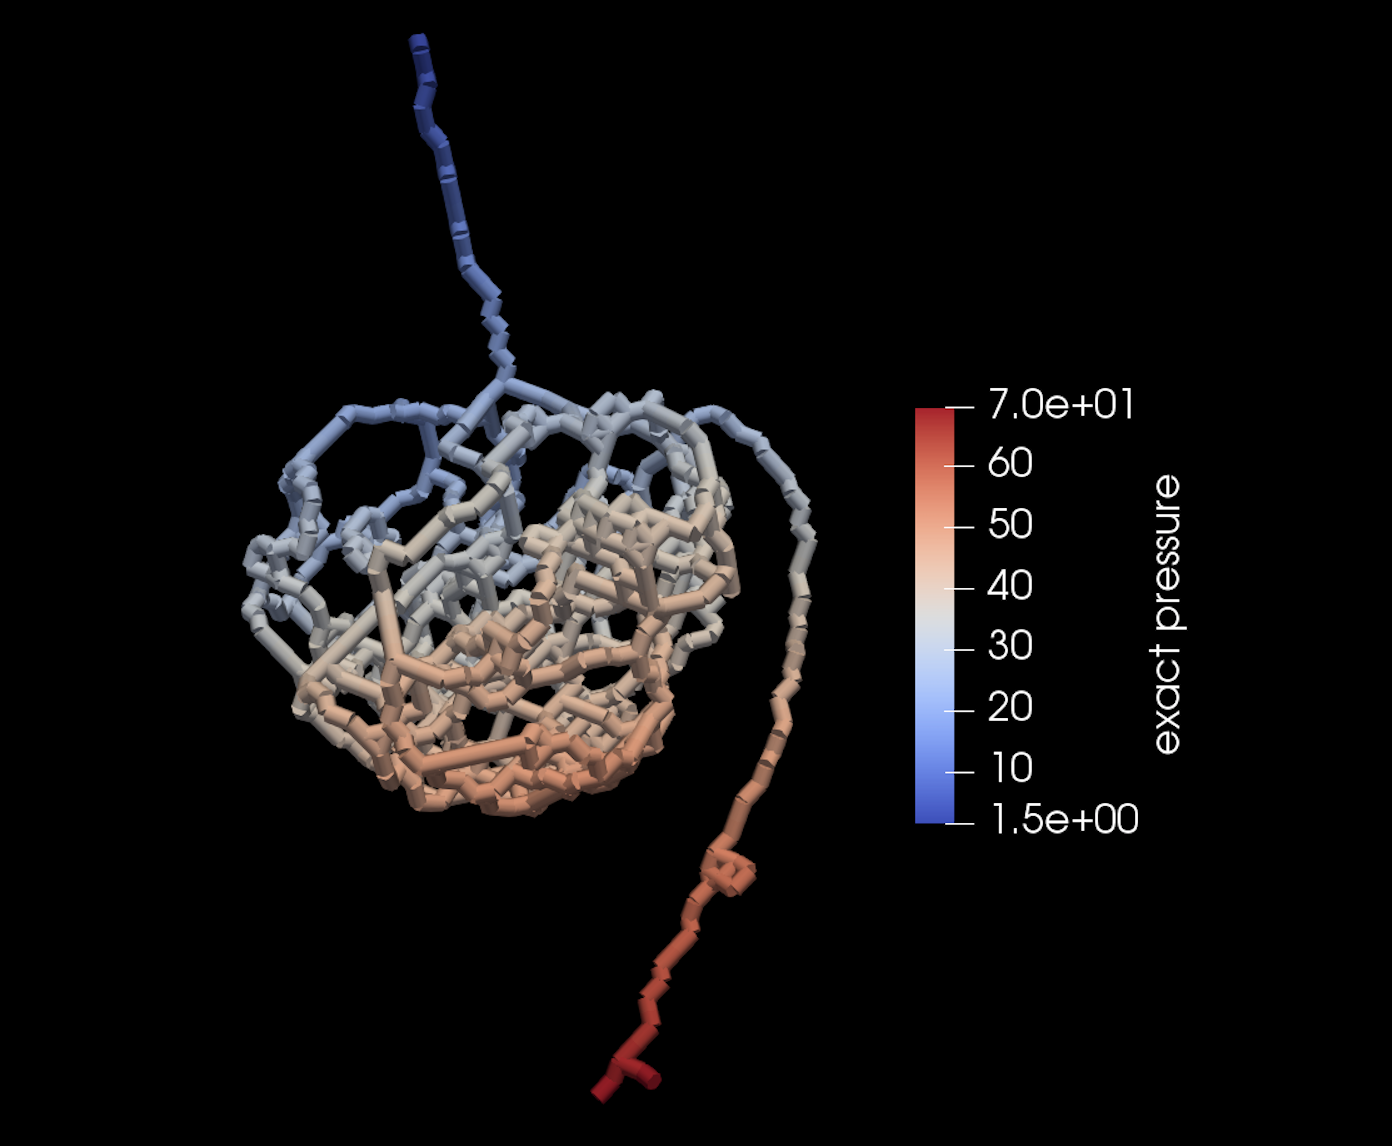
\includegraphics[width=162mm]{glom_pressure}
\caption{Pressure Field in Glomerulus 1}
\label{fig:glom_pressure}
\end{figure}
\begin{figure}[h]
\centering
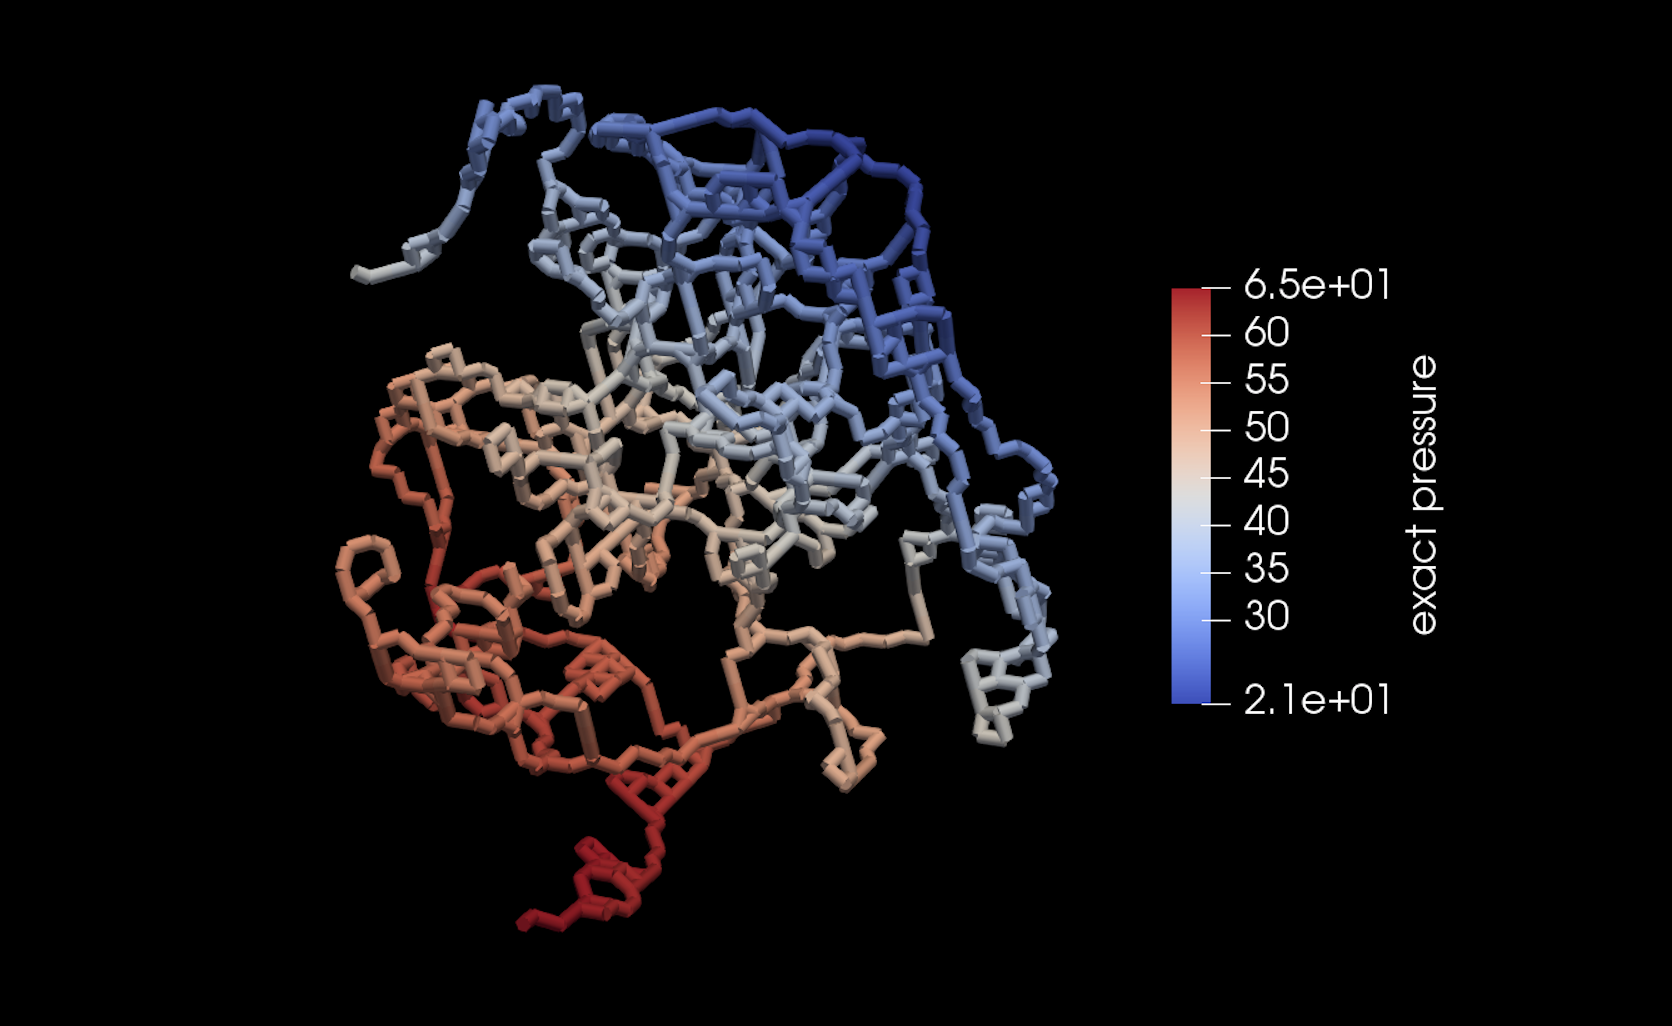
\includegraphics[width=162mm]{glom2_pressure}
\caption{Pressure Field in Glomerulus 2}
\label{fig:glom2_pressure}
\end{figure}
\begin{figure}[h]
\centering
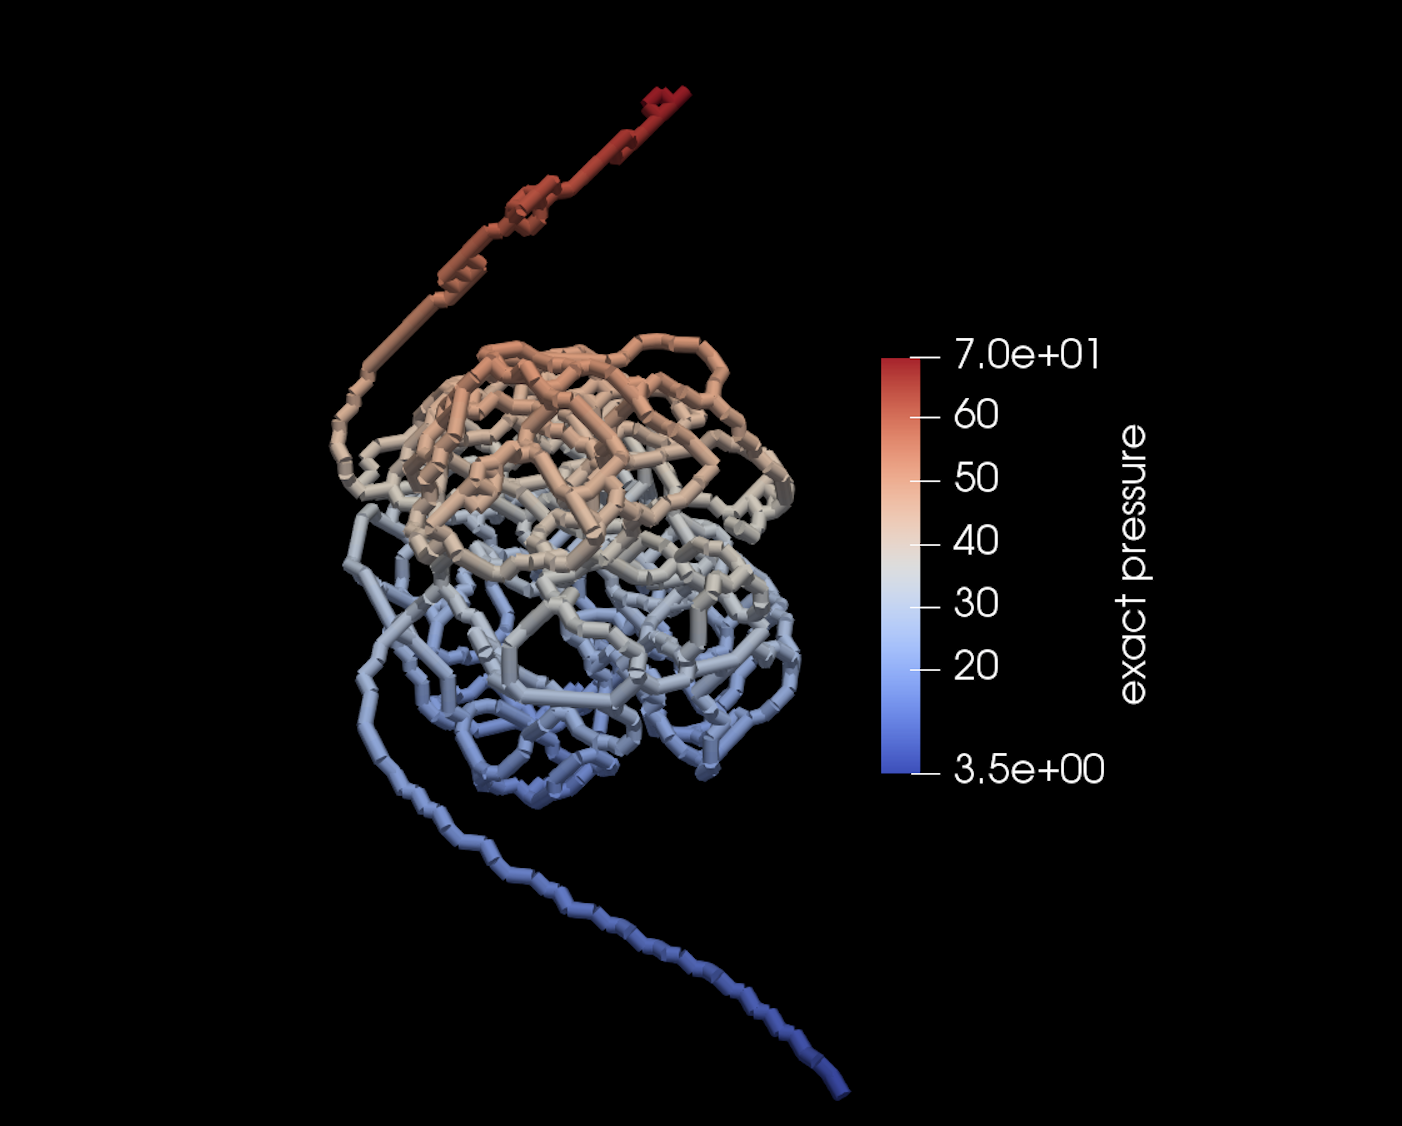
\includegraphics[width=162mm]{glom3_pressure}
\caption{Pressure Field in Glomerulus 3}
\label{fig:glom3_pressure}
\end{figure}
\begin{figure}[h]
\centering
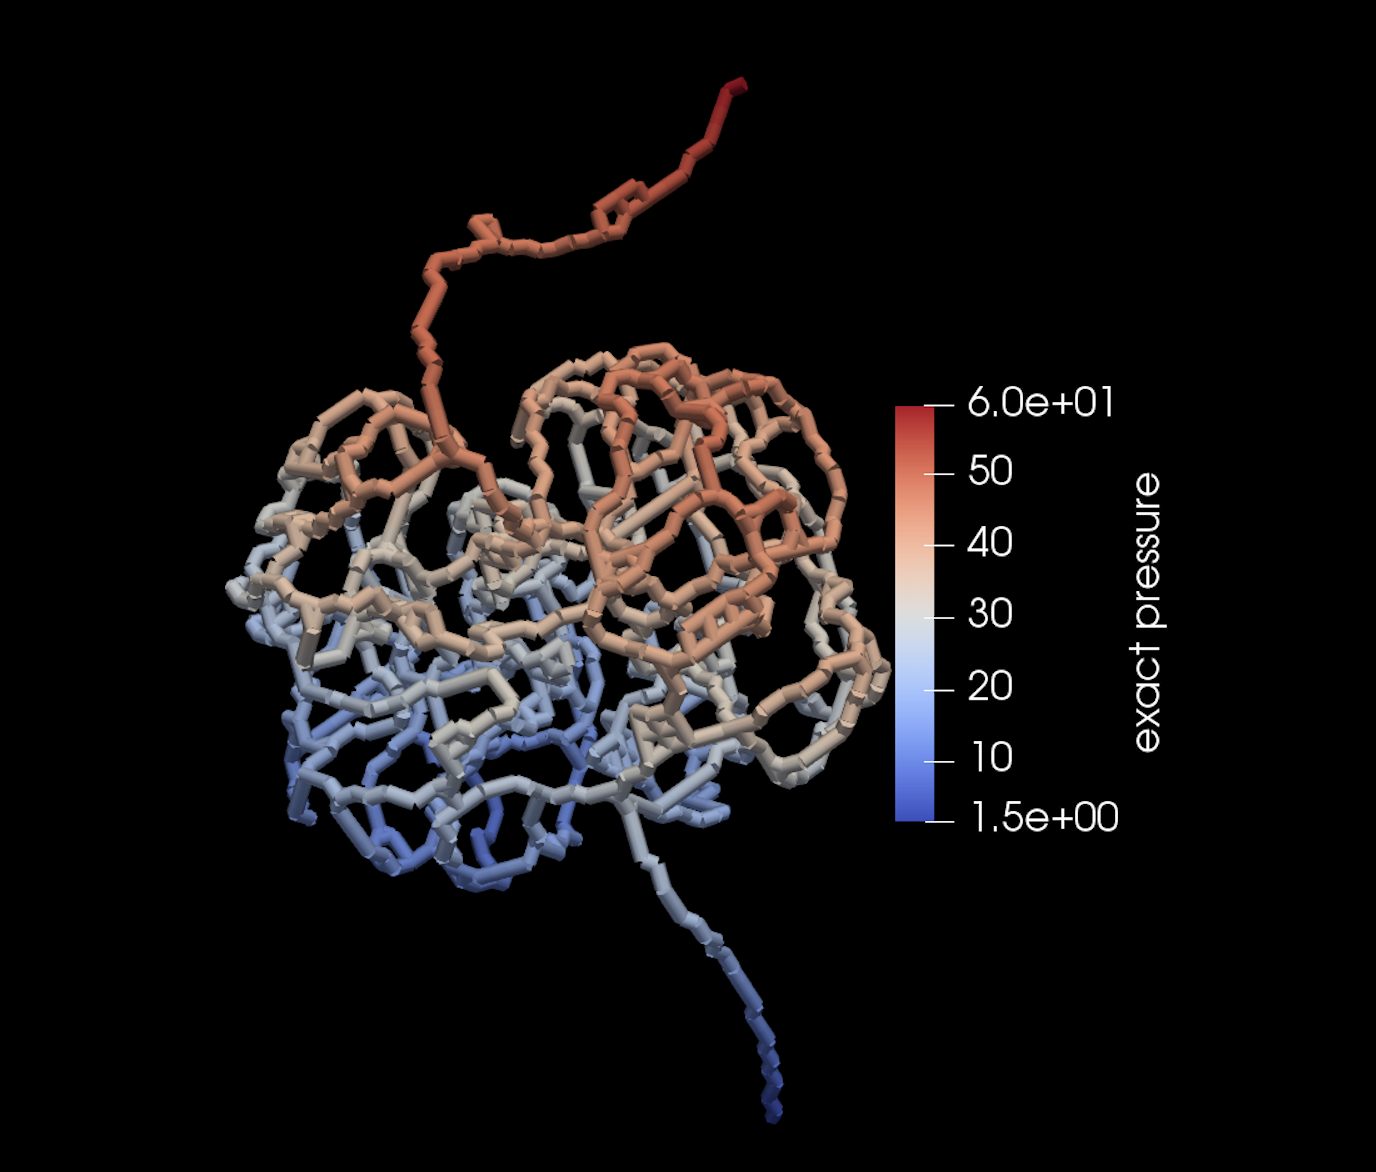
\includegraphics[width=162mm]{glom4_pressure}
\caption{Pressure Field in a Glomerulus 4}
\label{fig:glom4_pressure}
\end{figure}\\
The figures \ref{fig:glom_pressure},  \ref{fig:glom2_pressure},  \ref{fig:glom3_pressure} and  \ref{fig:glom4_pressure} are results of $DuMu^x$ blood flow simulations using the 1p-1p model in order to compute the pressure field inside the vessels of different glomeruli networks. The pressure field of the flow is visualized, where red is a relatively high pressure, and blue a relatively low pressure.\\
\\The figure \ref{fig:glom_pressure} shows a clear pressure drop in the flow direction for Glomerulus 1. The pressure drop takes place rather constantly over the glomerular network, and pressures fall from around $70$ mmHg down to less than $10$ mmHg. This pressure drop can be observed with a slightly different range of pressures for the glomeruli 2, 3 and 4. \footnote{The
pressure drop is qualitative as initial conditions were heuristically chosen.
Future work should apply a pressure profile at the afferent arteriole and then
compute the pressure gradient between efferent and afferent arteriole.}
\\
\\Physiologically, this pressure drop can be explained by the fact that the afferent arteriol, which is the vessel for the incoming blood, has a bigger diameter than the efferent arteriol, which is the vessel carrying the blood away from the glomerulus. From a simple engineering point of view, a bigger diameter for the outgoing flow results in a \emph{relaxation} of the fluid, and thus results in a pressure drop. By that we can say that the computational results of the 1p-1p model are physiologically correct.
\\It is possible to observe the same pressure drop when analyzing the pressure field in Glomerulus 2, and the rather constant fall in pressure is physically correct. A constant fall in the pressure is also what we would expect in a straight pipe. For this glomerulus, I would like to point out the fact that due to imaging artifacts and post-processing of the data, arterioles of this particular glomerulus seem to be missing, and thus these parts look rather short, but can still be seen on the figure. An especially interesting point is the fact that some vessels inside the glomerulus and the glomerular network have lower pressures than the pressure computed for the efferent arteriol. This can also be seen for Glomerulus 3 (figure \ref{fig:glom3_pressure}) and Glomerulus 4 (figure \ref{fig:glom4_pressure}).
\\Generally, it is possible to observe that the pressure constantly drops over the afferent and the efferent arteriols, before and after the glomerular network respectively. This pressure drop happens due to viscous effects and is proportional to the length, which explains the constant pressure drop. As previously mentioned, the afferent arteriol has a bigger diameter than the efferent arteriol in average, which causes an overall pressure difference from a physiological point of view. It is hard to understand the local pressure gradients inside segments of the glomerular network between the afferent and efferent arteriols, which might be due to diameter changes and in particular due to the complexity of glomerular networks in general.
\\

\subsubsection*{Results of the Implemented Method}
\label{ResultsImplMeth}

As I already briefly mentioned this when describing this method, the 1p-1p-tracer model cannot produce useful results yet. This new model in which I coupled the 1p-1p model with a new tracer model is basically still in the build-up phase, and with more time, the reasons for the wrong outputs can eventually be resolved so that the model can produce physically accurate results.
\\After spending a lot of time on debugging the errors I was having, the code finally compiled and the tracer could compute the oxygen distribution in my network (see \ref{fig:1p-1p-tracer-tracer-1} for a specific insight into the code that was used). However, the results are not satisfying as the oxygen concentration is computed to be zero at every time step in every node of the grid. The reasons for this are still not quite clear and some more investigation has to be made in order to understand why the tracer always has null values as outputs. Moreover, the initial and boundary conditions for the oxygen concentrations were examined and this seems not to be the source of the error.
\\As $DuMu^x$ is generally a complex software, many errors can occur, and it will surely take some time to understand the underlying problems in order to produce results using this model. However, I am persuaded that this approach can and will produce good results once the coupling of the models works well.

\newpage
\subsection{Comparison of the Methods and Results}
%Compare the produced results
In this section the main differences in the produced results by the Green's function method and $DuMu^x$ models will be discussed for networks of similar complexity.\\
%\\General differences in terms of computational cost and implementation issues can be discussed here as well when explaining the differences in the results.
\\Before starting, I would like to mention that oxygen fields computed on the same networks cannot directly be compared, as the $DuMu^x$ method (1p-1p-tracer-tracer) couldn't produce useful results yet, and thus no oxygen field in the tissue was computed. Additionally, the Green's function method didn't produce results on the Glomerulus 1 network either, which shows how hard it is to reproduce results using different methods in general.\\
While the Green's function method is presenting a specifically created C++ based software for oxygen transport and diffusion simulations, the results show that the obtained outputs can be very interesting for many heterogeneous and complicated networks. Unfortunately, oxygen fields could not be computed on every arbitrary network that was used, which raises the question of when and how the Green's method can produce results in general, in terms of oxygen field computations in the tissue.\\
\\Compared to this, the $DuMu^x$ based model is still in its very initial phase and cannot produce correct results yet. However, due to the fact that it is a $DuMu^x$ based model, it offers both a large flexibility to the user in terms of further development, as well as in terms of computational flexibility when choosing a time- and space-discretization through choosing discretization modules and different grid creators. The solvers can also be chosen by the user, which doesn't guarantee an overall stable numerical solver, but can provide great flexibility when adapting the model to specific networks.\\
\\Both the Green's function method and the $DuMu^x$ based 1p-1p model produced physically accurate results, which proved that they can be used to compute physiologically relevant results. Finally, the two methods currently compute entirely different entities, which is oxygen concentrations for the Green's method and overall pressure field for the $DuMu^x$ based 1p-1p method, and as the 1p-1p-tracer-tracer model is still in the build-up process, the results of the two different softwares used for this thesis cannot directly be compared for the moment.

%\\As seen previously, the ideas behind the Green's function method and the implemented $DuMu^x$-based method can offer very interesting options. While the Green's function method has proved its capabilities concerning oxygen field computations, the $DuMu^x$ based model couldn't produce results yet. I personally still believe that in the future this model can be optimized in order to compute oxygen fields in vascular networks and for the tissue surrounding it.\\
%\\As mentioned previously, one of the huge advantages of $DuMu^x$ is the flexibility it provides in terms of solvers, and thus in terms of the numerical methods used for the computations. This means that it is often possible to pick a solver which is stable for the specific problem and the chosen discretization.
%\\
%\\This is different for the Green's Method code, as there is no option of choosing a different solver than the one provided in the code. As discussed previously, this code is specifically implemented to solve and compute oxygen concentrations in the blood and the surrounding tissue, and the implemented method strongly relies on the stability of the Green's Method and the numerical methods behind the solver.

%\\EXPLAIN WHAT WAS COMPUTED WITH WHAT METHOD (PRESSURE VS. OXYGEN FIELD)
%\\EXPLAIN IF RESULTS RATHER GOOD OR BAD FOR EACH (DUMUX VS. GREENS)
%\\EXPLAIN THAT METHODS ARE VERY DIFFERENT, PRINCIPLES ARE COMPLETELY DIFFERENT, DUMUX MORE FLEXIBILITY AND THUS HAS MORE POTENTIAL FOR THE FUTURE, STILL HASN'T PRODUCED ANY OXYGEN COMPUTATION YET

%%%%%%%%%%%%%%%%%%%%%%%%%%%%%%%%%%%%%%%%%%%%%%%%%%
%\newpage
%\section{Comparison of the Different Methods Behind the Simulations}
%Compare DuMuX to Green's Method in general
%In this section the main differences between these two simulation methods described previously will be discussed.
%\\
%\\\textbf{Kartik do you think I need this 5th chapter at all ? I think I would rather delete it. I could include the subsections into the Simulation Methods part as well, and discuss some of these in the Conclusion as well ?}\\
%Compare the Solvers behind the Methods
%Very useful tu use Secomb Paper Numerical Methods section here
%\\In this section the main differences between the solvers and the associated numerical methods will be discussed.

%\subsection{Comparison of the Numerical Methods}
%Explain the Methods and differences between methods
%Very useful tu use Secomb Paper Numerical Methods section here
%In this section, the focus will be on comparing the numerical methods behind the Green's Method code and $DuMu^x$ and the differences in their implementation.

%\subsection{Stability Questions and Computational Cost}
%Explain when and why which the numerical methods are stable
%In this section, the consequences of the previously described differences will be discussed. The focus lies on the differences in terms of stability and computational cost for similar simulations.

\newpage
\newpage
\section{Discussion}
%Summary of both methods in general and Outlook for the research field
%What this review was about: short summary. Main points
%highlighted. Perhaps a graph regrouping together elements.
%Comparison of different strategies and their state. Maybe your own
%thoughts on the whole story and where the promising directions lie
%and which ones you see with scepticism.

This thesis aimed to understand how computational methods can be used to simulate blood flow and oxygen transport in microvascular networks. For this, two approaches have been presented \ref{Greens}, \ref{$DuMu^x$} and the results or outlooks have been discussed \ref{Results}.\\
\\While oxygen transport is a crucial topic in the fields of medicine and physiology, many processes in microvascular networks are not understood yet. Especially the measurements of microvascular and tissue oxygen concentrations is an uncharted research field. For this reason, a lot of research is being done in oxygen distribution computations \cite{goldman2001computational, lee2017accounting, kreuzer1982oxygen, secomb1993analysis} . In view of the challenges that are faced when simulating oxygen fields in tissue surrounding vessel networks, I would like to split this last section into three parts: a technical discussion, a physical discussion, and finally a physiologic discussion.

\subsection{Technical Aspects}
%- All the challenges one has to face when simulating in general
%- Computational problems in general
%- Flexible options given through simulating and computing thing we couldn't calculate otherwise (pressure in a kidney for example)
%- Things that are good about computational models

As the main tools used for the previously presented simulation results are computational solvers, I would like to focus on the technical aspects behind these tools in general.\\
\\The share computational simulations are taking in physiologic research is growing everyday. This is also due to the fact that some data is very hard to extract from measurements, and thus researchers try to understand certain processes through running computational simulations on physical models. However, the challenges behind using these technical tools are not to be underestimated. As I experienced myself when running simulations with the Green's method code \ref{Greens} and $DuMu^x$ \ref{$DuMu^x$}, many errors and bugs can stop the code from running and can be very hard to fix. Also, once a model is implemented, one has to take great care to examine if the produced results physically make sense. As for example for the $DuMu^x$ model I implemented, the zero outputs are clearly wrong and the model has to be improved in order to produce realistic results \ref{ResultsImplMeth}.
\\The reason computational models are used so frequently is also due to the fact that some calculations, like the pressure gradients in the previously presented glomeruli \ref{ResultsDum}, can not be obtained without computational methods. This is especially due to the particular vasculature of these networks. Thus, these tools can give us very interesting insights, even though their complexity is certainly challenging, and will demand a good understanding of the methods underlying, depending on the used software.

\newpage
\subsection{Physical Aspects}
%- Resume the physics behind the problem
%- Explain what outputs were generally produced and physically discuss things like pressure drops
%- Say why engineers are also interested in this field and that the fluiddynamics in the body are very interesting in general

As the exact physical equations and mathematics behind the different simulation methods was explained in the first sections, it was obvious that the success of computational simulations is strongly linked to the correctness of the physical assumptions.\\
\\When building a computational model like the models used in this thesis, one has to start by studying the physical equations describing the given problem \ref{CompMod}. In our case, the physical equations describing the blood flow, and accordingly the oxygen transport from the vessel to the tissue have been used in general. Solving these equations will then yield the results that the user wanted to compute \ref{Results}. This basic procedure is an engineering procedure, and is the same for a flow and heat exchange computation in a pipe or a blood flow and oxygen diffusion computation in a tissue. Due to this fact, engineers are strongly engaged in this research field, as they have a good knowledge about the technical tools and have a good understanding for physical quantities. Also, the used networks and fluiddynamic challenges can be very interesting in the physiology field, as for example the flow in a complex vascular network like the one found in glomeruli \ref{ResultsDum}, where particularly interesting pressure differences and gradients could be observed. To understand and analyze these results physically, a deeper understanding of the Navier-Stokes equations is required, as the pressure drop was not comparable to the one in a straight pipe.\\
\\Due to these reasons, engineers, mathematicians and physicists are and will be used more and more often in these research domains in the future, as some physical problems can not be solved without computational methods to this day.

\subsection{Physiological Aspects}
%- Again what is going on in the body exactly
%- Why do we want to know this
%- Give some examples from the results and explain what is physiologically happening in blood flow and oxygen transport\\

Finally, I would like to give a short outlook to the research done in this thesis from a physiological point of view.\\
\\As the methods and the produced outputs were presented in the previous sections \ref{Methods}, \ref{Results}, one could clearly see that the computed results were physiologically very interesting. With computed oxygen concentrations ranging from $0$ mmHg to around $87$ mmHg in the tissue, the values seemed realistic and the distributions inside the tissue seemed to be qualitatively correct. The pressure gradients computed by the $DuMu^x$ model \ref{$DuMu^x$} were also analyzed and the general pressure field could physiologically be explained. Again, we do not really have experimental values to compare the computed values with, so most of the results can only be analyzed qualitatively.
\\Especially the oxygen fields computed by the Green's method \ref{Greens} in some complex networks produced very interesting and physiologically useful results \ref{ResultsGreens}. Even though we don't have experimental data to compare the computational values with, it is possible to see that the results were all in the physiologic range and the general oxygen distribution showed that the outputs were in accord with the physics describing our problem \ref{CompMod}. Extrapolating from the examples presented for oxygen distribution computations, I would like to underline the fact that computational models are very useful in this specific field and will very likely take an even more important share in the future.
\\
%\\Main conclusions and final remarks.

%\section{Conclusion}
Main conclusions and final remarks.


% Bibliography
\newpage
\addtocontents{toc}{\vspace{.5\baselineskip}}
\addcontentsline{toc}{section}{\protect\numberline{}{References}}
\bibliography{article}


% Appendices (if needed)
\addtocontents{toc}{\vspace{.5\baselineskip}}
\appendix
%!TEX root = article.tex

\section{Appendix}
\label{s:Appendix}

Additional material such as extra figures.

\subsection{Additional Material for the Green's Function Method}
%Put all the extra plots etc. from Green's Function Code here.

\subsubsection{General Structure of the Used Code}
%Explain everything about the code

In this section, an insight to the code provided by Secomb et al. \cite{Secomb2004} will be given. Especially some explanations about what data this code uses and what data it computes will be given. 
The main goal is to understand what the results are, how correct their accuracy is. For this, a general explanation of the structure and organization of the code and the methods behind the computations will given.

\subsubsection*{Inputs}
\label{Inputs}
%What data this code actually needs and what this data is

What are the inputs for this code ? Where do they come from ?
\\
\\The Green's Function Method takes .dat-files as inputs, which basically contain the network files.
\\
The input data in form of .dat-files is basically build out of four files:
\\- SoluteParams.dat: This file contains all the information about the solutes we are looking at. This information can be things like tissue solubility, Michaelis constant of consumption, etc.
\\- Network.dat: This file contains all the information about the network we are looking at. This information is basically in form of an array. This array defines for each segment the type, the start point, the end point, the diameter (in microns), the relativ flow (?) and the hematocrit (?).
\\- IntravascRes.dat: This file contains all the information about a diameter (which one?) and the intravascular resistance to radial oxygen transport K for each diameter/vessel.
\\- ContourParams.dat: This file contains all the information necessary to create the contour-plots. This means that we create a plot, where the oxygen concentration can be visualized on a 2-dimensional slice. (not sure how plot is created from this data?)
\\
\\The part of the code where the read-in of the network data and the sources (not sure about this) through the input files is being done is the input.cpp code.
\\
\\The analyzenet.cpp-part of the code analyzes the input-files...

\subsubsection*{Outputs}
\label{Outputs}
%What this code actually produces

What are the outputs for this code ? How are they produced ? Where do they come from ?
\\
\\The Green's Function Method gives .dat-files and images (contour.ps-files) as outputs, which basically contain the results that will be discussed later in the next chapters.
\\
\\The contour.ps-files are produced by the contour.cpp-part of the code, which basically generates and writes the data for the contour-plots. This data is a plot of the vessel from bottom to top according to the z-coordinate. One could see this plot as a 2D picture of a 3D network when looking from the bottom. A new pages is generated for each solute, and the computed solute concentration for each area is shown in colors.
\\
\\picturenetwork.cpp: picturenetwork.cpp - project network on z = 0 plane.
Uses parameters from CountourParams.dat
Labels nodes with nodvar and segments with segvar (must be float).
Generates a postscript file.
\\
The general outputs of the code can be classified into two categories:
\\- The first category is in the form of PostScript-files that can be visualized similar to pictures.
\\- The second category is in the form Text-files, containing the computed data.
\\

\subsubsection*{Organization of the Code}
%Briefly talk about each part of the code and explain how it all works together
%Might keep this part more general and mention each of the parts of the code like a puzzle in the Appendix

The code provided by Secomb et al. \cite{Secomb2004} consists of a few .cpp-files, so that tasks like input read-ins, calculations and output-file generations are separated. Each file has a specific role, which will be explained in detail in this section. As one can think, the most important part of this code is the implementation of the Green's Function Method and its application to the given data.
\\
%Solver bicgstab
\\The bicgstab.cpp-part of the code is the implementation of a solver based on the Parameter-free iterative linear solver by R. Weiss \cite{weiss1996parameter}.
\\
%blood
\\The blood.cpp-part of the code is quite interesting, as it basically does an important part of the calculation to obtain the oxygen concentration and distribution in the vessels and the tissue. In this part of the code
\\
%contr-lines
\\The contr-lines.cpp-part of the code generates the contour lines for these plots, whereas the contr-shade.cpp-part of the code generates the colors and the color bar on the side of the generated picture/plot.
\\
%convect
\\The convect.cpp-part of the code does the convective (flow) part of the calculation.
\\
%eval
\\The eval.cpp-part of the code does the evaluation of the solute field depending on the source strengths provided.
\\
%numerical methods (gaussj and ludcmp)
\\There are some numerical methods and mathematical calculations behind the simulation, as for example the Gauss-Jordan elimination or the Lower-Upper decomposition, which is implemented in the gaussj.cpp-part and the ludcmp.cpp-part of the code.
\\
%greens
\\The main implementation of the Green's Function Method is in the greens.cpp-part of the code, where Green's Function approach for multiple reacting species is implemented. (Talk more about this, heart of the code)
\\
%histogram
\\Histograms of solute levels are evaluated in the histogram.cpp-part of the code.
\\
%initgreens
\\Initial tissue source strengths (given uniform solute field) are computed in the initgreens.cpp-part of the code.
\\
%main
\\The code main.cpp calls the greens.cpp-code.
\\
%nrutil (.cpp and .hh)
\\The code nrutil.cpp/nrutil.hh is declaring variables and is allocating them.
\\
%outboun (method?)
\\Outboun.cpp: method = 1: finds the smallest convex region inside the cuboid
which excludes tissue node points that have a distance to the nearest
vessel greater than a value specified by the user (lb).  Any point
outside a region between two planes containing the required points is
excluded.  This is repeated for multiple plane orientations, determined by am.
\\
\\method = 2: finds all tissue points within a distance lb of the vessels, but
does not make a convex region.  Fills in 'holes' in interior, whether 2D or 3D.
\\
\\Output:	nnt, total tissue node points inside the region.
nbou > 1 if inside region, value gives tissue point index
\\
%putrank
\\putrank.cpp: generate nodes in order of flow direction
\\
%readsources
\\readsources.cpp: read source strengths from file (from TissueSources.out and VesselSources.out)
\\
%setuparrays 0, 1, 2
\\setuparrays0.cpp: set up arrays with fixed dimensions (for Green's)
\\
\\setuparrays1.cpp: set up arrays with dimensions of nnod and nseg (for Green's)
\\
\\setuparrays2.cpp: set up arrays with dimensions of nnv and nnt (for Green's)
\\
%testconvect
\\testconvect.cpp: testing if convect is giving correct results for alpha (?) matrix. Comparing matrix values with values obtained by numerical differentiation.
\\
%tissrate
\\tissrate.cpp: computing tissue uptake rates of solutes as a function of solute levels (concentration)
\\
\\Everyone of these code-parts is using the nrutil.hh code, why ?

\subsubsection{Some More Green's Results}

Figure \ref{fig:Contour_Cardiac}  is the result of a Green's Method blood flow simulation computed on a Cardiac network. The Solute Concentration in the network is visualized.\\
\begin{figure}[h]
\centering
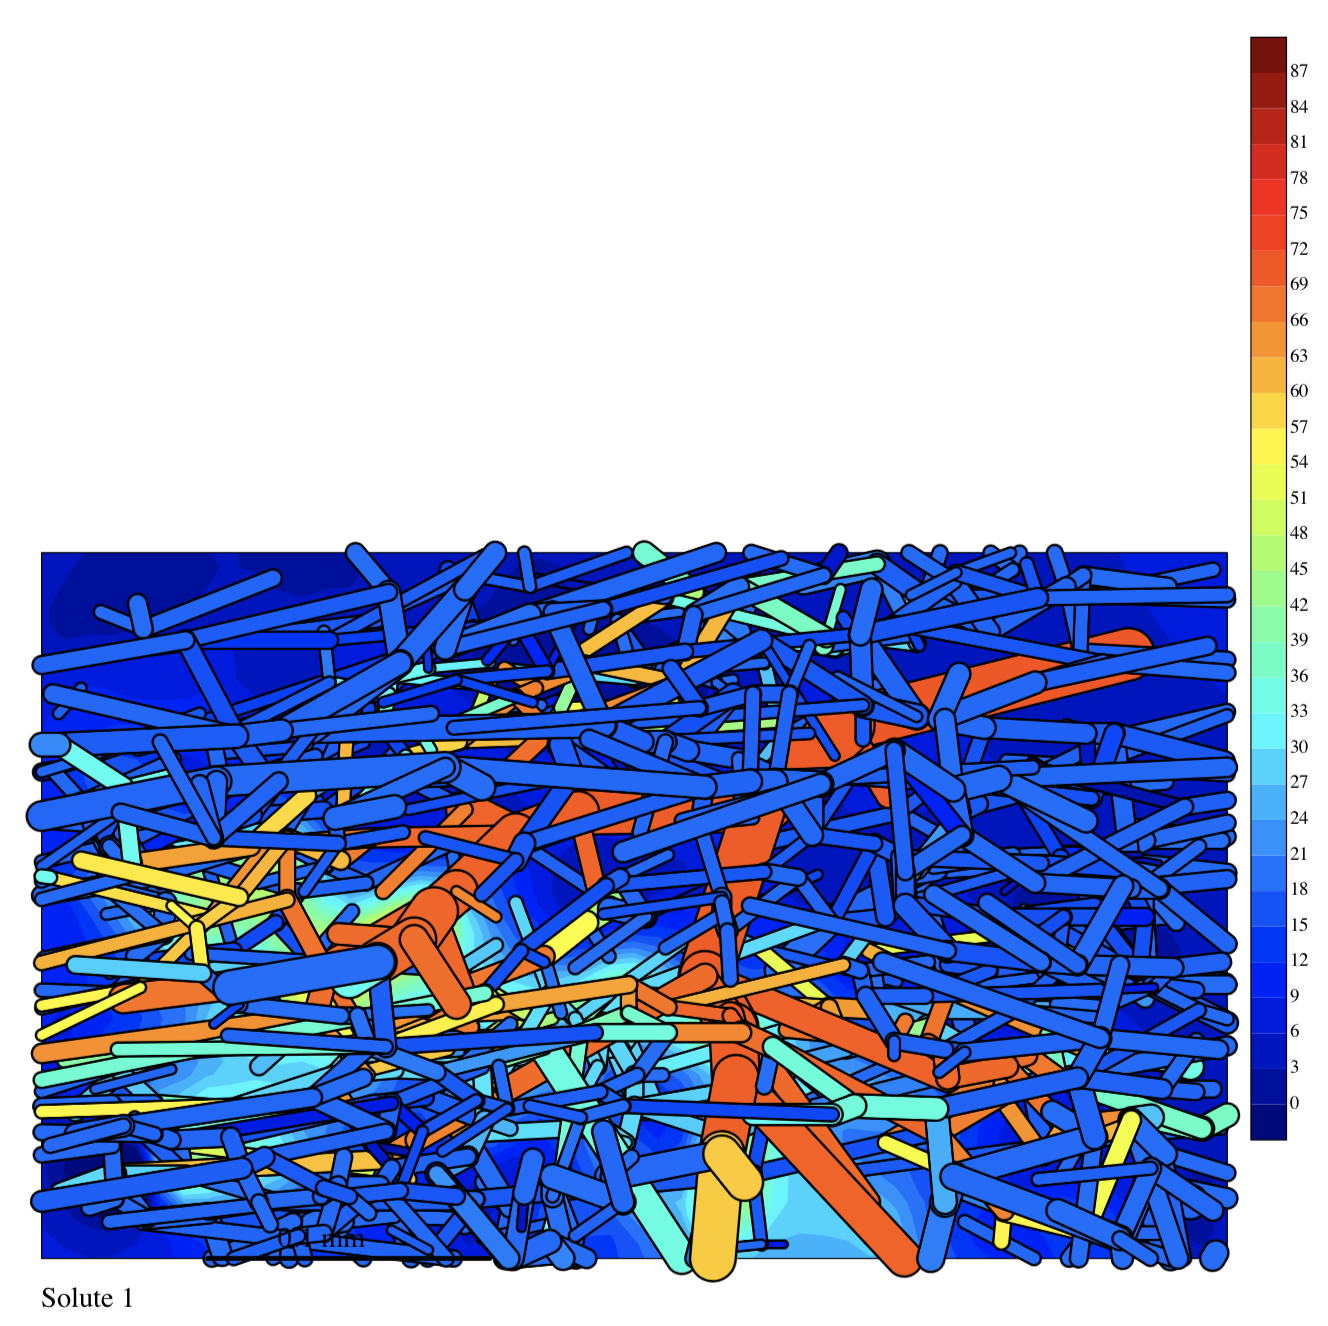
\includegraphics[width=170mm]{Contour_Cardiac}
\caption{Green's Contour Output for Cardiac Network}
\label{fig:Contour_Cardiac}
\end{figure}

\subsection{Additional Material for DuMuX}
%Put all the extra images from ParaView here.

\newpage
\subsubsection{Some Glomerulus Network Simulation Results}
%Just to have some more figures

\begin{figure}[h]
\centering
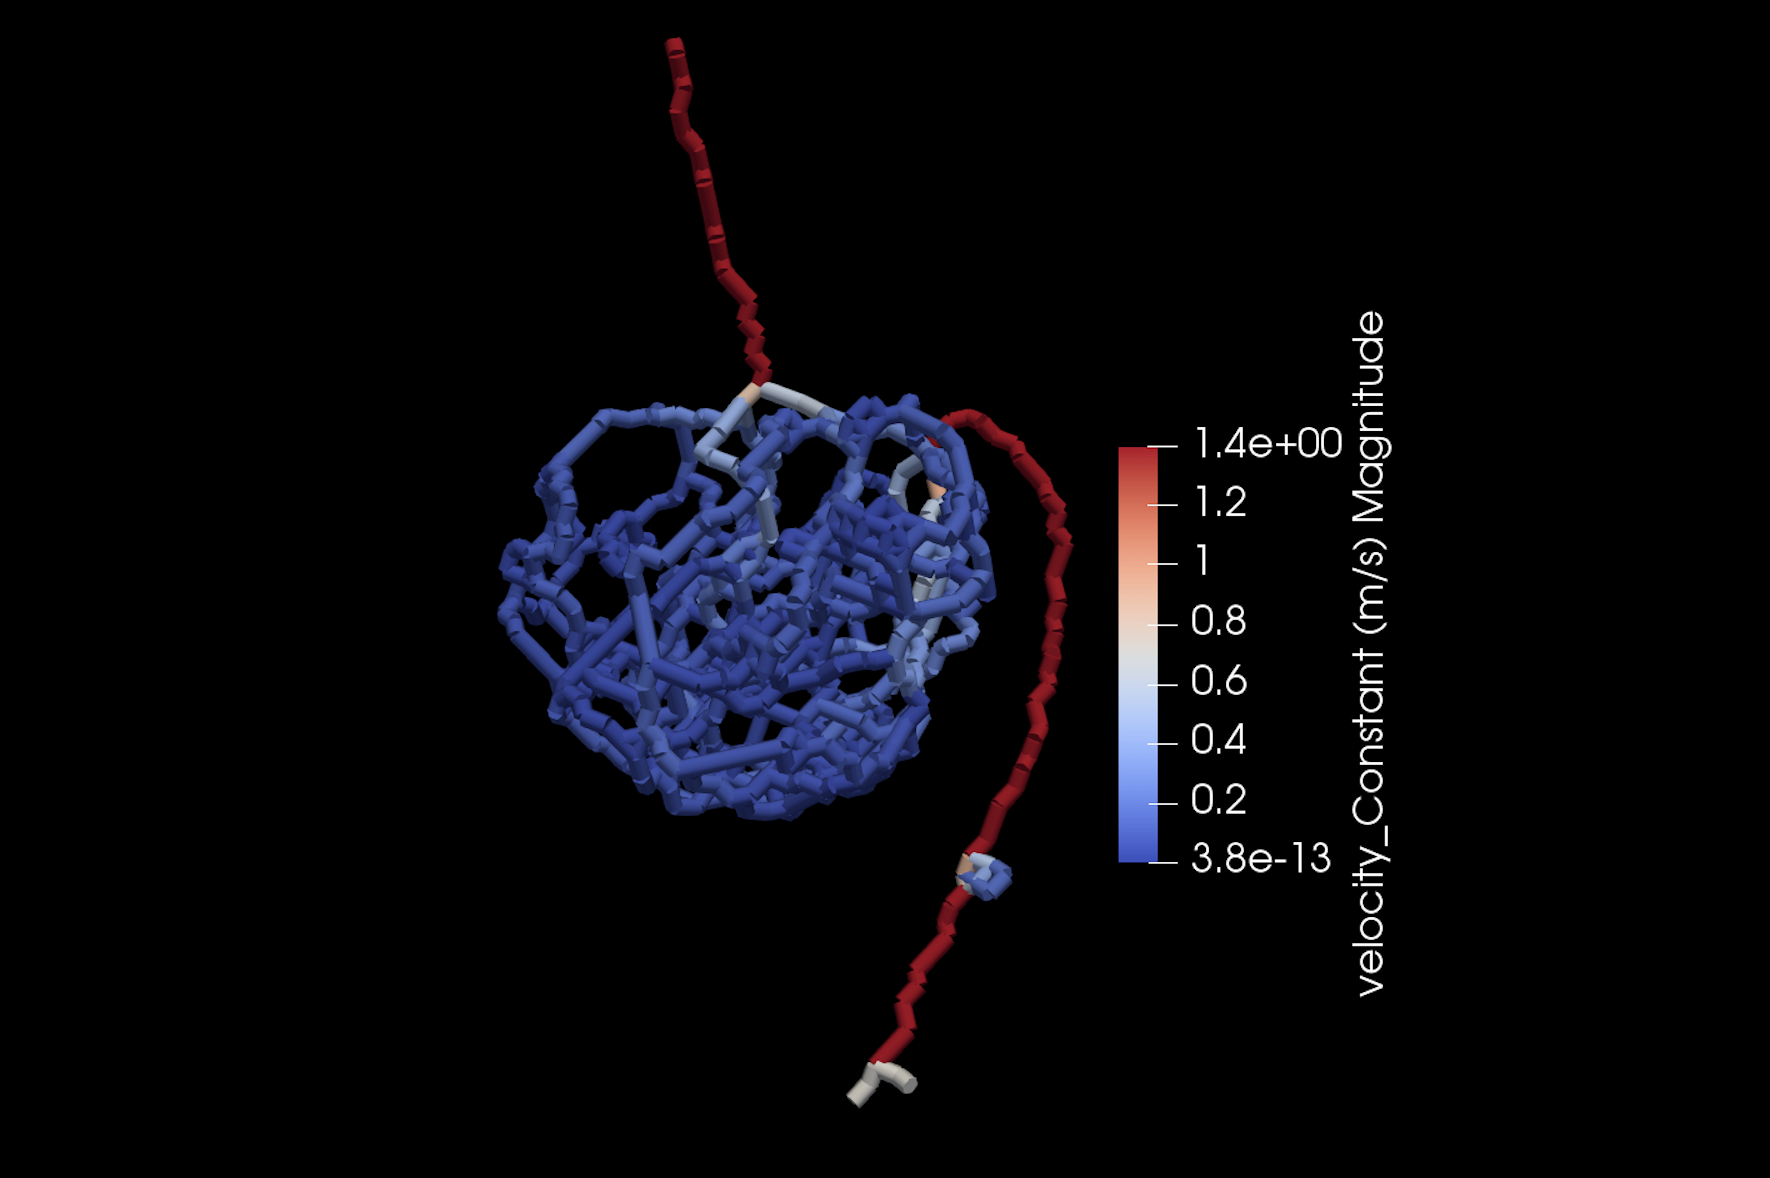
\includegraphics[width=162mm]{glom_velocity}
\caption{Velocity Field in a Glomerulus}
\label{fig:glom_velocity}
\end{figure}
The figure \ref{fig:glom_velocity} is the result of a DuMuX 1p-1p blood flow simulation computed on a glomerulus network. The velocity field of the flow is visualized.\\

\begin{figure}[h]
\centering
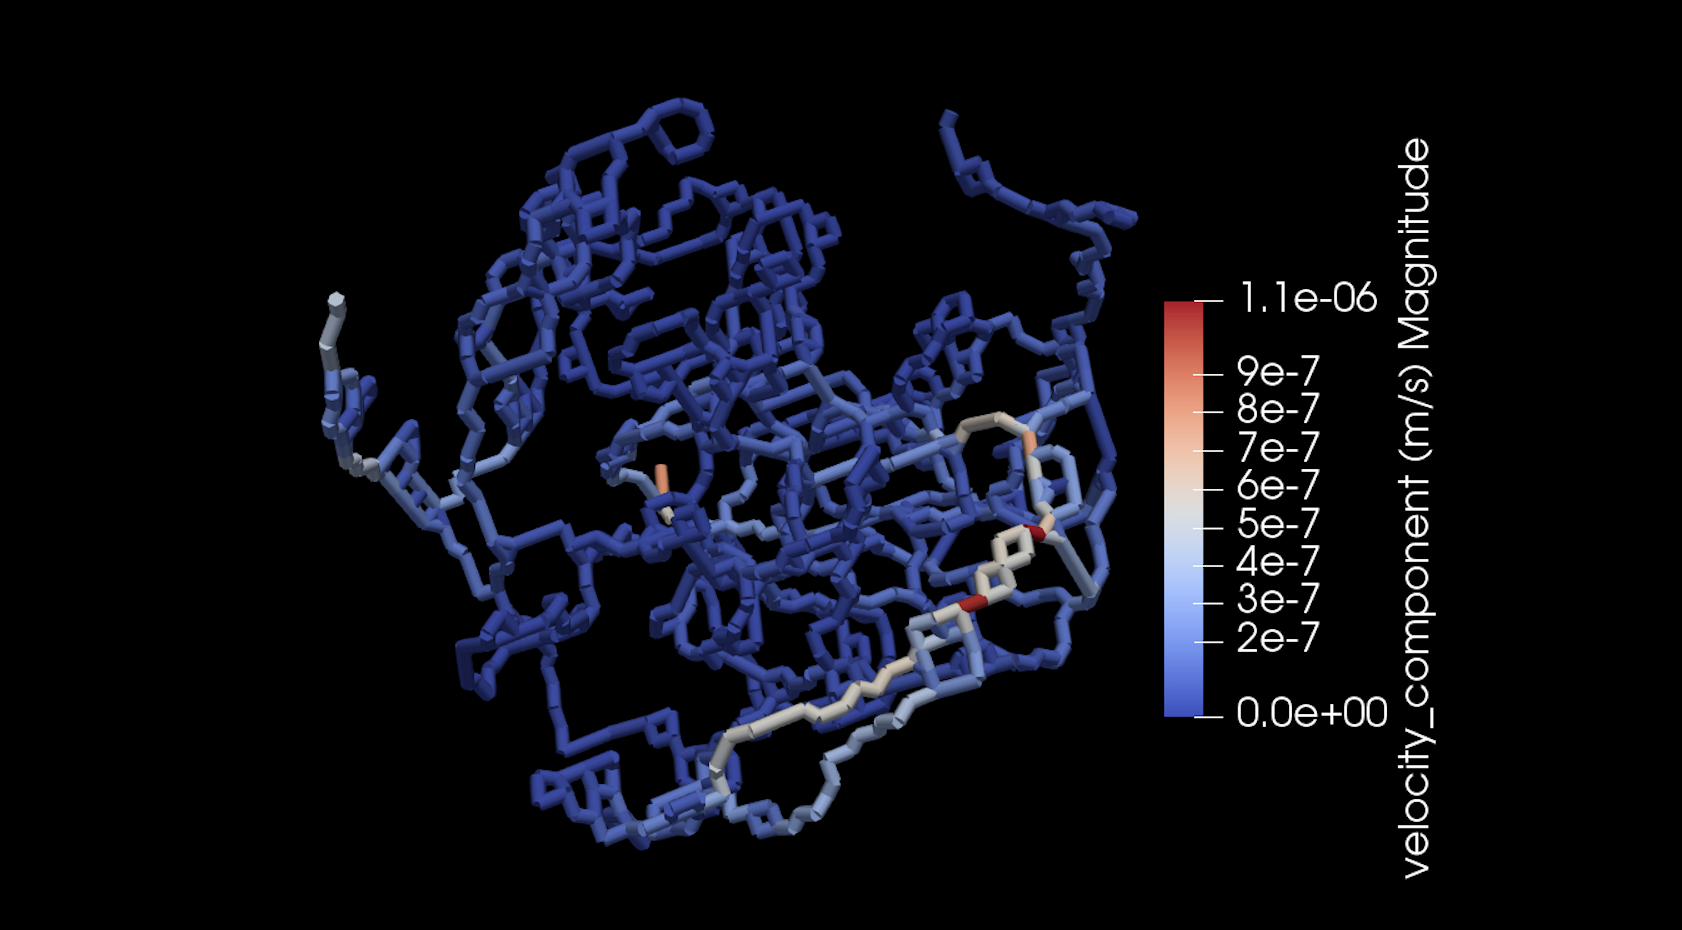
\includegraphics[width=162mm]{glom2_velocity}
\caption{Velocity Field in a Glomerulus}
\label{fig:glom2_velocity}
\end{figure}
The figure \ref{fig:glom2_velocity} is the result of a DuMuX 1p-1p blood flow simulation computed on a glomerulus network. The velocity field of the flow is visualized.\\

\subsubsection*{Some Tracer Simulations}

\begin{figure}[h]
\centering
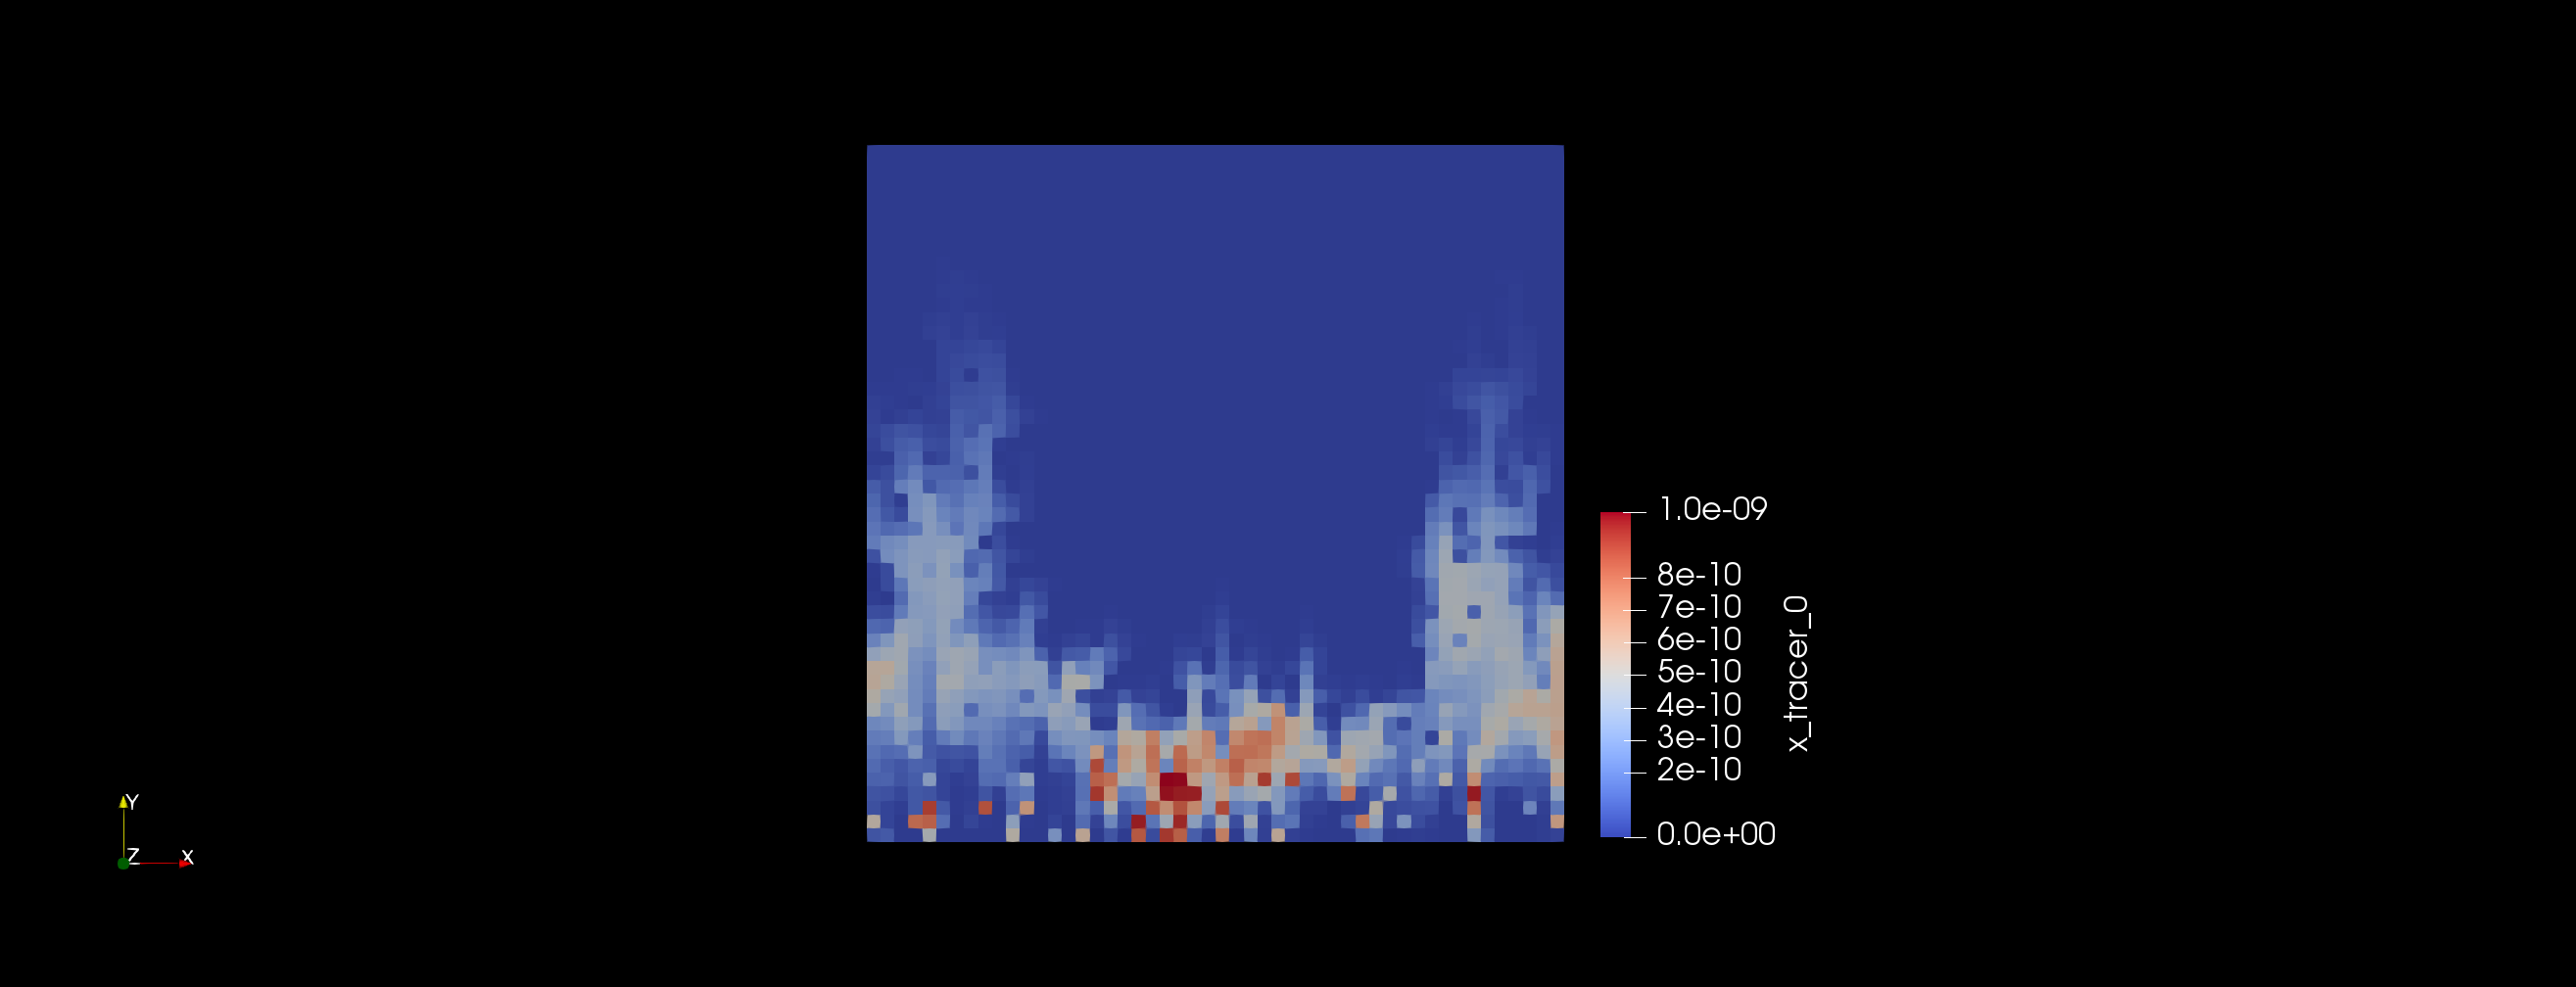
\includegraphics[width=162mm]{tracer_1}
\caption{\footnotesize $DuMu^x$ Tracer Concentration Simulation for a Rectangular Geometry (Time Step 1)}
\label{fig:tracer_1}
\end{figure}
Figure \ref{fig:tracer_1} is the result of a $DuMu^x$ tracer simulation computed on a rectangular geometry. The solute field in the network for the first time step is visualized.\\
\begin{figure}[h]
\centering
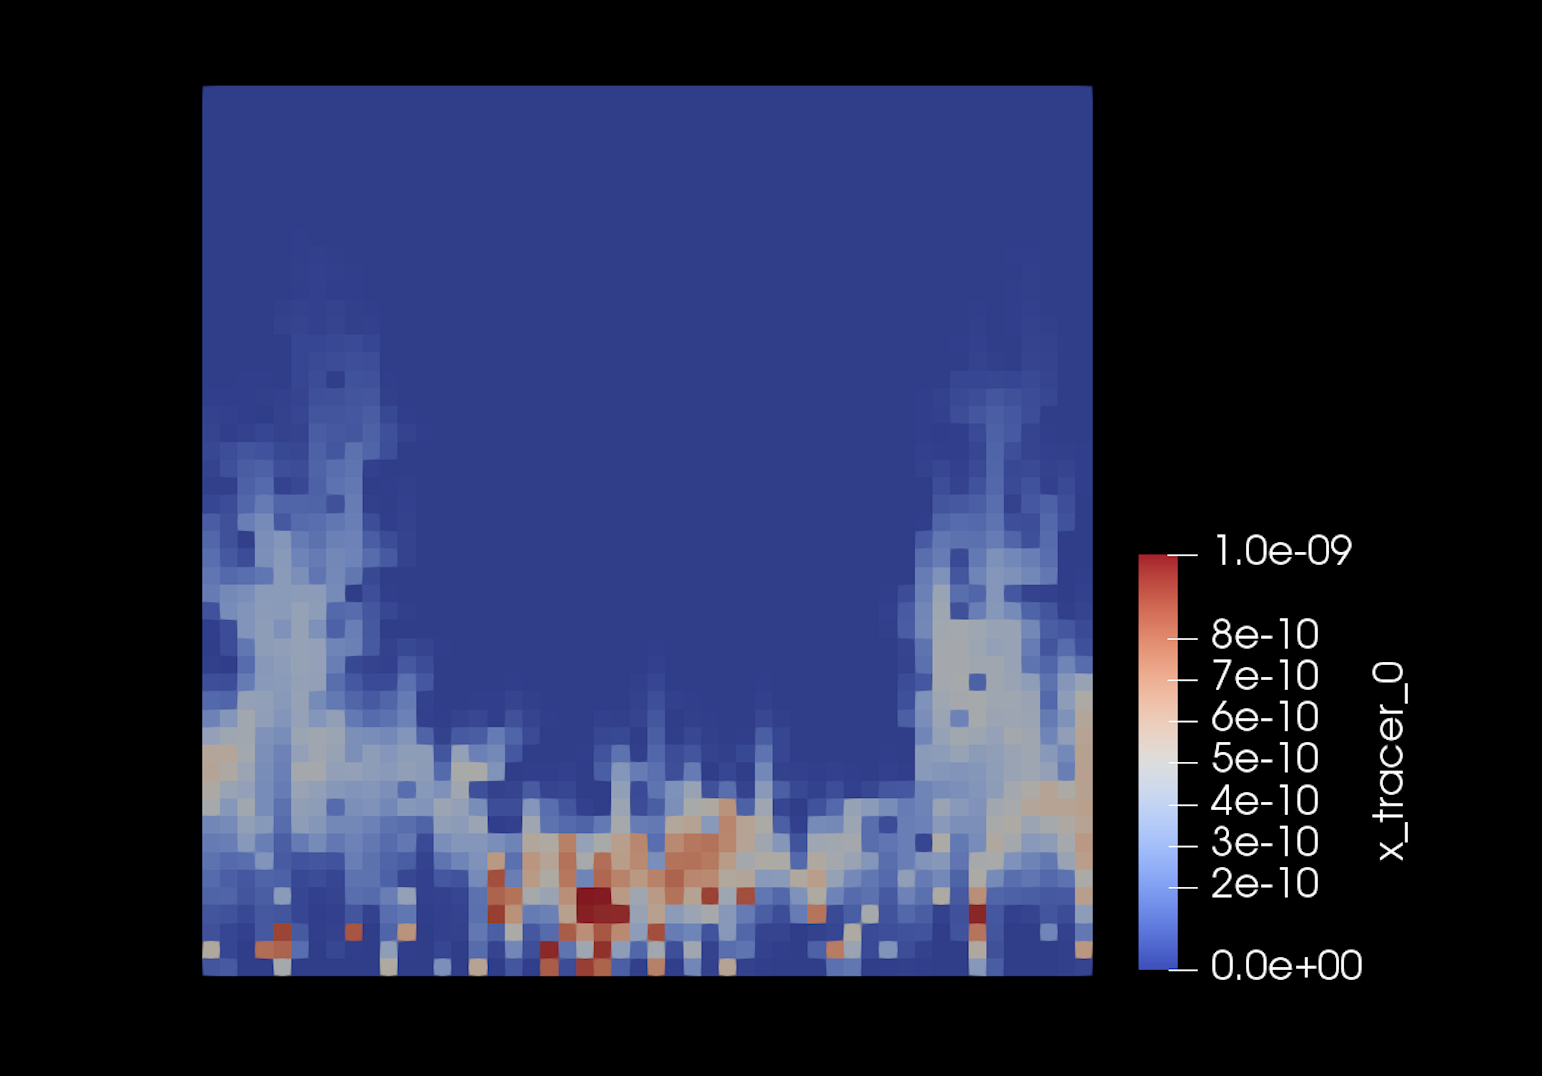
\includegraphics[width=162mm]{tracer_2}
\caption{\footnotesize $DuMu^x$ Tracer Concentration Simulation for a Rectangular Geometry (Time Step 10)}
\label{fig:tracer_2}
\end{figure}
Figure \ref{fig:tracer_2} is the solute field for the same simulation for the last time step is visualized.\\
\begin{figure}[h]
\centering
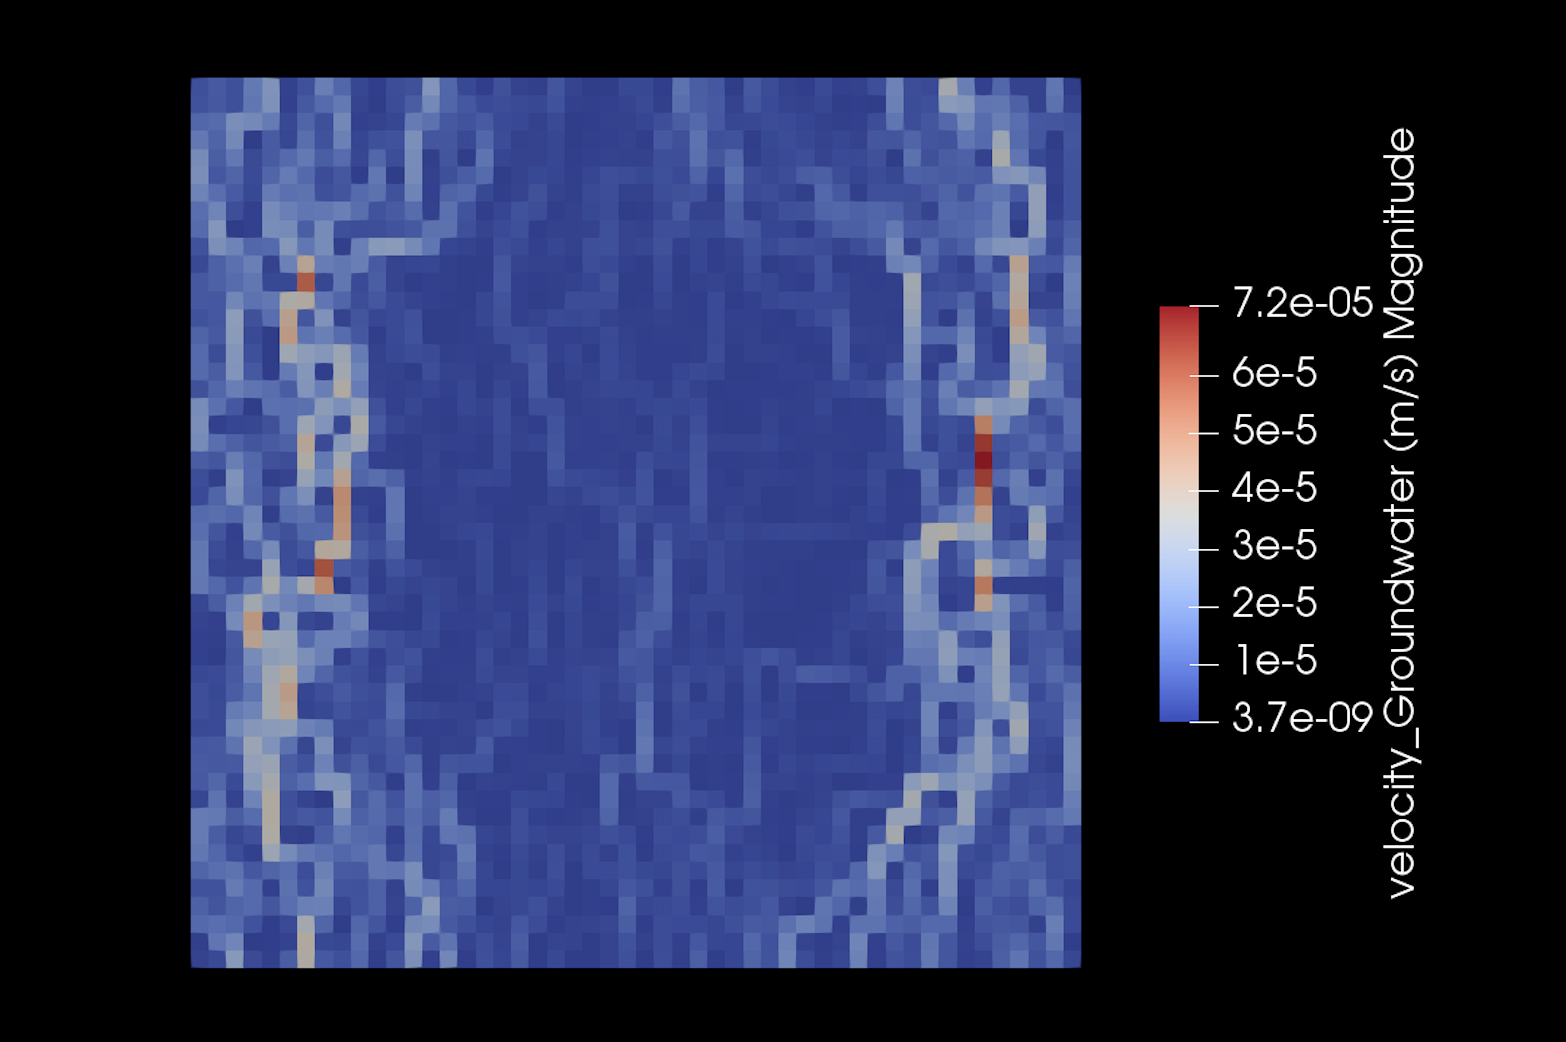
\includegraphics[width=162mm]{tracer_velocity}
\caption{\footnotesize $DuMu^x$ Tracer Velocity Simulation for a Rectangular Geometry}
\label{fig:tracer_velocity}
\end{figure}
Figure \ref{fig:tracer_velocity} is the constant velocity field of the solute.\\
%\section{Examples}
\label{s:Examples}

This appendix provides some additional hints and examples for the
layout and style of the thesis. It is worthwhile to look at the source
file \verb|Examples.tex| for this appendix to understand how it was
created.



\subsection{Tables}

Tables are left justified and the caption appears on top as seen in
Table~\ref{t:Translations}.

\begin{table}[ht]
\caption[Translations]{\label{t:Translations}Translations.}
\begin{tabular}{ll}
\hline
\textbf{English} & \textbf{German}\\
\hline
cell phone       & Handy\\
Diet Coke        & Coca Cola light\\
\hline
\end{tabular}
\end{table}



\subsection{Figures}

Figure~\ref{f:IRISlogo} shows a simple figure with a single picture
and Figure~\ref{f:SubfigureExample} shows a more complex figure
containing subfigures.

\begin{figure}[ht]
\centering

\includegraphics[width=.6\linewidth]{IRISlogo}
\caption[IRIS logo]{\label{f:IRISlogo}IRIS logo.}
\end{figure}

\begin{figure}[ht]
\centering
\subfigure[ETH logo]{
\includegraphics[height=12mm]{ETHlogo}}\quad
\subfigure[IRIS logo]{
\includegraphics[height=12mm]{IRISlogo}}
\caption[Subfigure example]{\label{f:SubfigureExample}Two pictures as
  part of a single figure through the magic of the subfigure package.}
\end{figure}



\subsection{Units}

The SIUnits package provides nice spacing for units as demonstrated in
Table~\ref{t:SIUnits}. Use of the package also makes it easy to change
the style or even the unit text in the future.

\begin{table}[ht]
\caption[Spacing for units]{\label{t:SIUnits}Spacing for units.}
\begin{tabular}{ll}
\hline
\textbf{Output}   & \textbf{Command}\\
\hline
42m               & \verb|42m|\\
\unit{42}{\metre} & \verb|\unit{42}{\metre}|\\
42 m              & \verb|42 m|\\
\hline
\end{tabular}
\end{table}



\subsection{Miscellany}

\begin{description}

\item[Capitalization.] When referring to a named table (such as in the
  previous section), the word \emph{table} is capitalized. The same is
  true for figures, chapters and sections.

\item[Naming of structural elements.] Refer to a \verb|\section| in
  \LaTeX\ as a chapter and call a \verb|\subsection| section. (I don't
  like the way \verb|\chapter|s are rendered in the report document
  class. Hence the suboptimal markup/naming correspondence.)

\item[Bibliography.] Use \verb|bibtex| to make your life easier and to
  produce consistently formatted entries.

\item[Contractions.] Avoid contractions. For instance, use ``do not''
  rather than ``don't.''

\item[Captions.] A brief version of a caption can be provided for the
  list of figures and tables as demonstrated with the caption of
  Figure~\ref{f:SubfigureExample}. The mechanism can also be used to
  get rid of the final period of a caption in the lists.

\end{description}



\end{document}
